\chapter{Conception du système}

\section{Introduction}
%Of course talk here about what the chapter is about
\paragraph{}
Durant ce chapitre, nous allons présenter en détail les étapes de conceptions de notre système, tout d'abord une architecture générale est présentée et décortiquée, ensuite chaque module du système sera détaillé du point de vue des composants qui le constitueraient en donnant un maximum de détails tout en restant assez concis. Une conclusion viendra clôturer ce chapitre pour introduire ensuite le suivant.
\section{Architecture du système}
%Try to be as precise as possible while letting room for more details to the next sections
\begin{figure}[H]
	\centering
	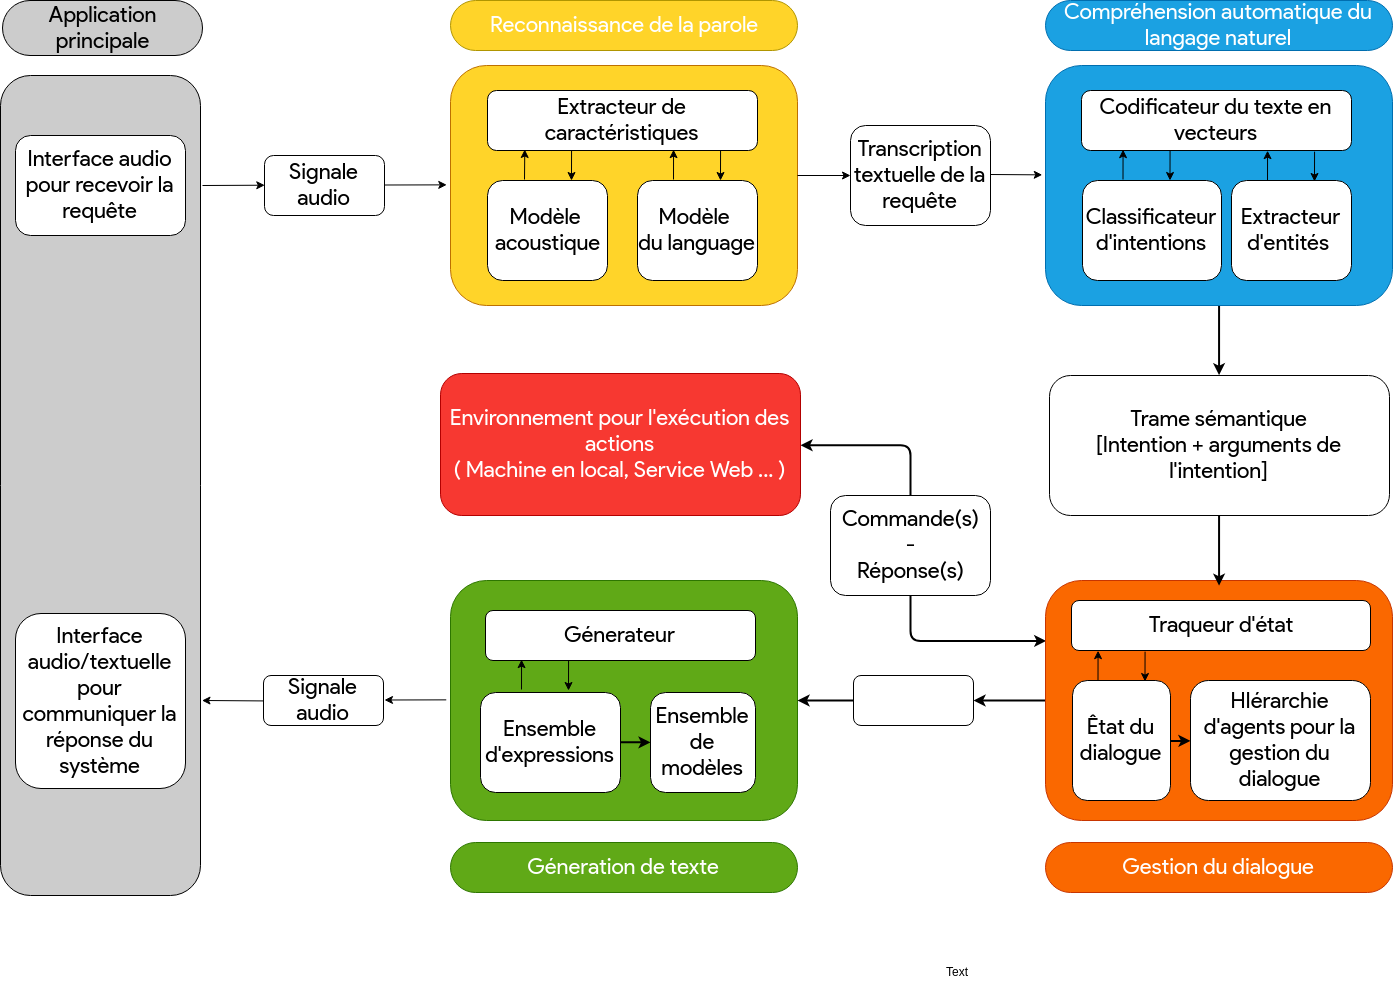
\includegraphics[width=0.87\linewidth]{images/SPA_architecture.png}
	\caption{Architecture générale de notre système}
	\label{spaArch}
\end{figure}
\paragraph{}
Comme montré dans la figure ci dessus (voir ~\ref{spaArch}) et comme cité dans le chapitre précédent (voir \ref{spaSchemSection}) le système se présente comme l'interconnexion de cinq parties dont une interface \footnote{Ici nous par interface nous entendons le sens abstrait du terme et non obligatoirement le sens interface graphique} et quatre modules internes, chaque module forme ainsi un maillon d'une chaîne qui représente une partie du cycle de vie du système. L'architecture du système est une pipeline (chaîne de traitement) de processus qui s'exécutent de manière indépendante mais qui font circuler un flux de données entre eux dans un format préalablement décidé (voir ~\ref{fig:spaDiagram}). Nous pouvons séparer ces parties en deux catégories :
	\subsection{Couche utilisateur}
%	What the users sees as input/output and the interfaces that are available for him
	\paragraph{}
	Cette couche représente ce que l'utilisateur peut voir comme entrée/sortie et les interfaces qui lui sont accessibles, puisque l'assistant est un processus qui communique majoritairement avec l'utilisateur à travers des échanges verbaux, nous avons pensé à implémenter l'interface du système comme une processus qui s'exécute en arrière plan et qui attend d'être activer (pour le moment par un événement physique, c.à.d clique sur un bouton/icône ou raccourci clavier), l'assistant pourra ensuite répondre en affichant un texte à l'écran qui sera vocalement synthétisé envoyer à l'utilisateur via l'interface de sortie de son choix (afficher le texte et sa transcription vocale pourrait palier au manque d'un périphérique de sortie audio).
	\subsection{Couche système}
	
%	What the users doesn't see and what are the main components of the system
	\paragraph{}
	\label{system_layer}
	Cette couche quant à elle représente ce que l'utilisateur ne voit pas et fait donc partie du fonctionnement interne du système, elle regroupe les quatre grandes étapes d'un cycle de vie pour une commande reçu de la couche utilisateur. Comme mentionné dans le chapitre précédent (voir \ref{spaLifeCycle}), la requête passe par un module de reconnaissance de la parole, qui traduira en texte le signale audio correspondant à la requête, le module suivant va extraire l'intention de l'utilisateur et ses arguments (par exemple \textit{"open the home folder"} pourrait donner  une intention dy type  \textit{open\_file\_desire[file\_name="home",parent\_directory="?"]}), le gestionnaire de dialogue gardera trace de l'ensemble des échanges effectués entre l'utilisateur et l'assistant et essayera d'atteindre le but final formuler par la requête (la plus récente ou la plus ancienne), pour ce faire il aura besoin d'interagir avec ce qu'on a appelé un environnement d'exécution, qui peut être la machine où l'assistant réside ou une API \footnote{Application programming interface ou interface de programmation applicative } qui aura accès à un service a distance (sur internet par exemple) ou locale (dans un réseau domestique). Finalement une action spéciale qui servira à informer l'utilisateur sera envoyé au module suivant pour être transformé en son équivalant en langage naturel, puis le texte sera vocalement synthétiser et envoyé vers l'interface de sortie de l'application.
	
	\paragraph{}
	Nous allons maintenant détailler la conception des différents modules en précisant à chaque fois le ou les processus de sa mise en œuvre. 
\section{Module de reconnaissance automatique de la parole}
\paragraph{}
Premier module du système, il joue un rôle clé dans la véridicité du dialogue entre l'utilisateur et la machine, en effet il devait être assez robuste et précise dans la transcription de la requête en entrée minimiser les erreurs et les ambiguïtés qui peuvent survenir dans le reste de la pipeline. C'est pour cela que nous avons décidé de ne pas développer un sous-système en partant de zéro, par faute de temps et par soucis de précision nous avons décidé de nous baser sur un outil open-source nommé DeepSpeech \cite{deepspeech_paper}, naturellement du fait que ce soit un projet open-source nous avons pu avoir accès à différentes informations concernant le modèle d'apprentissage, d'inférence et la nature des données utilisé pour le premier et le teste du deuxième.
	\subsection{Architecture du module}
	\paragraph{}
	Le module possède une architecture en pipeline dont chaque composant exécute un traitement sur la donnée reçu par son prédécesseur
	\begin{figure}[H] 
		\centering
		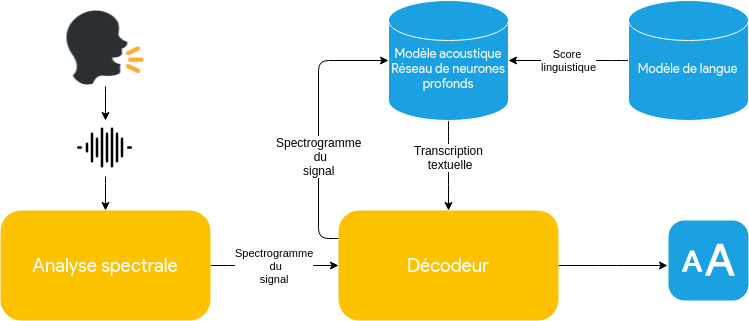
\includegraphics[width=0.88\linewidth]{images/Conception/ASR/schema.png}
		\caption{Architecture de notre module de reconnaissance de la parole}
	\end{figure}
	\subsection{Modèle acoustique}
		\subsubsection*{Type du modèle}
		\paragraph{}
		Le modèle d'apprentissage (qui est principalement le modèle acoustique à l'exception d'une partie consacré au modèle linguistique) possède une architecture en réseau de neurones avec apprentissage de bout-en-bout composé de trois parties : 
		\begin{itemize}
			\item Deux couches de convolution spatiale : pour capturer les patrons dans la séquence du spectrogramme du signal audio.
			\item Sept couches de récurrence (Réseaux de neurones récurrents) pour analyser la séquence de patrons (ou caractéristiques) engendré par les couches de convolutions. 
			\item Une couche de prédiction utilisant un réseau de neurone complètement connecté pour prédire le caractère correspondant à la fenêtre d'observation du spectrogramme du signal audio. La fonction d'erreur prend en compte la similarité du caractère produit avec le véritable caractère ainsi que la vraisemblance de la séquence produite par rapport à un modèle de langue basé sur les N-grammes (voir \ref{n-grams})
		\end{itemize}
		\begin{figure}[H] 
			\centering
			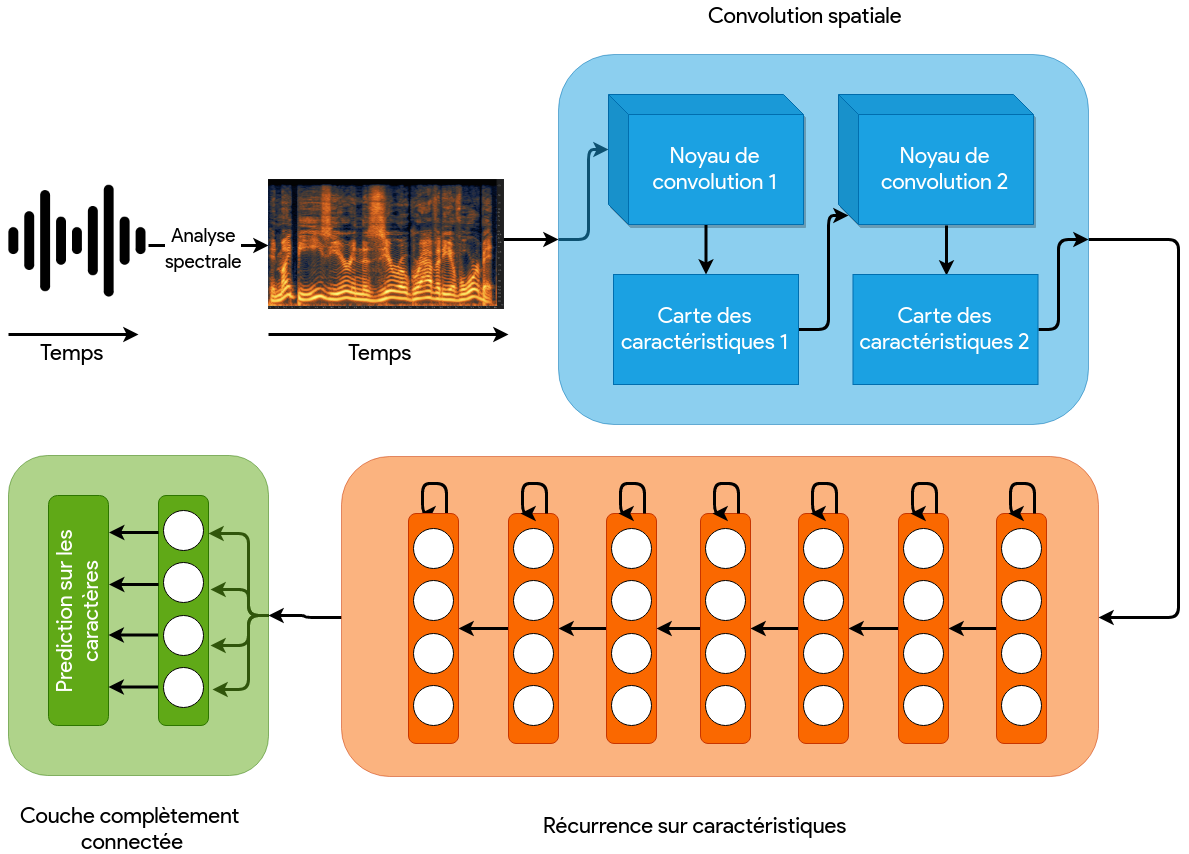
\includegraphics[width=0.88\linewidth]{images/Conception/ASR/deeps_speech_arch.png}
			\caption{Architecture du modèle DeepSpeech \cite{deepspeech_paper}}
			\label{fig:deepSpeechArch}
			
		\end{figure}
		\subsubsection*{Données d'apprentissage}
%		audio files and their transcriptions
		\paragraph{}
		Pour entraîner le modèle acoustique, Mozilla à lancé le projet Common Voice  \footnote{\url{https://voice.mozilla.org/fr}} une plateforme enligne pour récolter des échantillons d'audio avec leurs transcriptions textuelles, chaque lot (batch) de données reçu est alors manuellement validé par l'équipe de Mozilla pour l'inclure dans la banque de données d'exemples. À ce jour plus et pour la langue anglaise, la plateforme à récolté plus de 22Go de données, soit 803 heures d'enregistrement appartement à plus de 30 000 voix différentes dont 582 heures ont été validées. Mais ces données ne sont rien comparées à celle déjà utilisées pour l'apprentissage initial, en effet plusieurs source ont été combinées pour construire cet ensemble de données, dans \cite{deepspeech_paper} il a été mentionné que trois ensembles d'apprentissage existants ont étés utilisés dont WSJ (Wall Stret Journal) \footnote{\url{http://www.cstr.ed.ac.uk/corpora/MC-WSJ-AV/}}, Switchboard \footnote{\url{https://catalog.ldc.upenn.edu/LDC97S62}} et Fisher \footnote{\url{https://catalog.ldc.upenn.edu/LDC2004S13}} qui cumulent 2380 heures d'enregistrements audio en anglais et plus de 27 000 voix différentes, vient s'ajouter à cela l'ensemble Baidu \footnote{\url{https://ai.baidu.com/broad/introduction}} avec 5000 heures d'enregistrements et 9600 locuteurs.
		
	\subsection{Modèle de la langue}
		\subsubsection*{Type du modèle}
		\paragraph{}
		Pour ce qui est du type du modèle de langue, c'est un modèle basé sur les N-grammes (3-grammes pour être plus précis) qui est utilisé, en effet il permet de façon assez simple et intuitive de capturer l'enchaînement des mots dans une langue donnée, rendant ainsi la transcription assez proche de la façon dont les mots sont distribués dans le corpus d'apprentissage.
		
		\subsubsection*{Données d'apprentissage}
		\paragraph{}
		À l'origine, DeepSpeech utilise un modèle de langue dont la source n'est pas dévoilée par les chercheurs dans \cite{deepspeech_paper}, mais son volume est approximativement de 220 million de phrases avec 495 000 mots différents. Cependant puisque ce corpus nous reste inconnu et qu'il a probablement été construit pour reconnaître des séquence de mots de phrase en anglais assez générales, nous avons décidé de construire notre propre modèle de langue en récoltant des données depuis des dépôts sur le site \href{https://github.com/}{Github}, plus précisément les fichiers README.md des dépôts qui font office de manuels d'utilisation d'un projet hébergé sur le site, ce type de fichier renferment généralement des instructions de manipulation de fichiers, de lancement de commandes ..., ce qui offre un bon corpus pour le modèle de langue, car en effet notre système se concentre plus sur l'aspect de manipulation d'un ordinateur, donc la probabilité de trouver certaines séquences de mots qui appartiennent au domaine du Tech est plus élevé en théorie. La procédure suivi est la suivante : 
		\begin{figure}[H] 
			\label{lm_gathering}
			\centering
			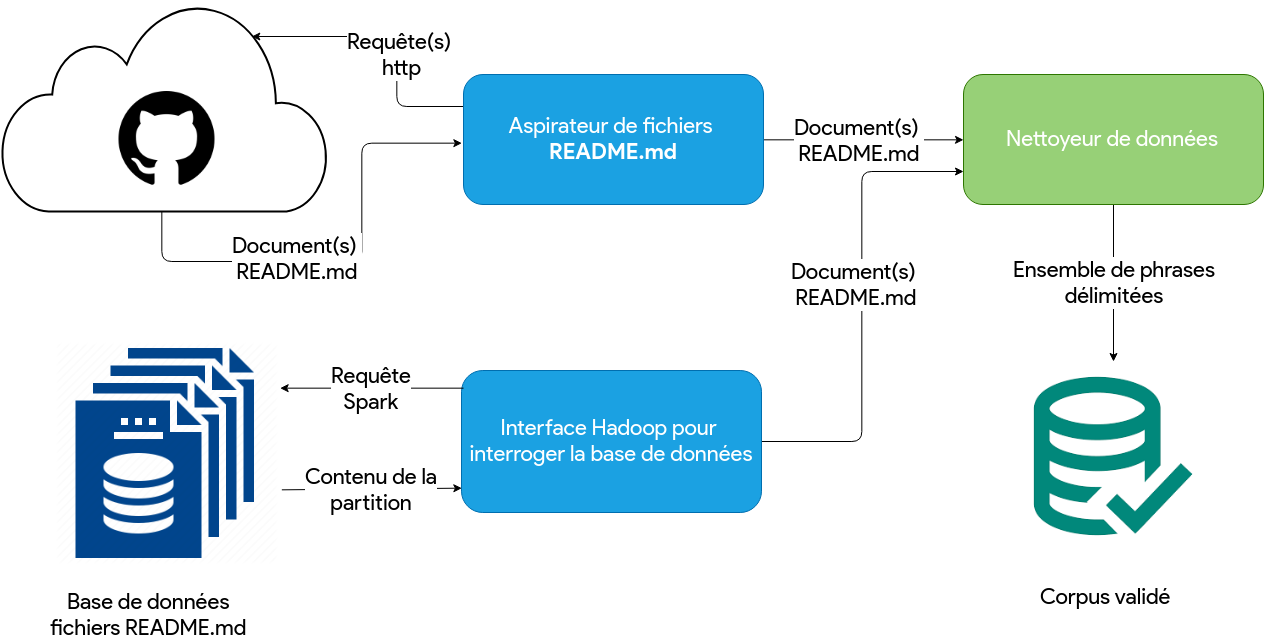
\includegraphics[width=0.88\linewidth]{images/Conception/ASR/lm_gathering.png}
			\caption{Processus de génération du corpus pour le modèle de langue}
		\end{figure}
		\newpage
		\begin{itemize}
			\item L'acquisition des données dans leur format brut \textbf{.md} (markdown) se fait de deux manières :
			\begin{itemize}
				\item Depuis le site officiel de GitHub en faisant des requêtes http au serveur en suivant le patron suivant des urls : 
				\begin{lstlisting}[language=python]
				'http://raw.githubusercontent.com/'+NOM_DÉPOT+'/master/README.md'\end{lstlisting}
				La liste des noms de dépôt est disponible dans un fichier \footnote{\url{https://data.world/vmarkovtsev/github-readme-files/file/top_broken.tsv}} en free open acces au format \textbf{.csv} dont les colonnes sont \textit{Nom\_Utilisateur} et \textit{Nom\_Dépot} 
				\item En lisant un base de 16 millions de fichiers différents dont la taille totale atteint 4.5 Go  
			\end{itemize}
			\item Les deux sources de données envoient ensuite les fichiers récoltés au nettoyeur de fichiers pour en extraire seulement les parties qui ont du sens (c.à.d paragraphes, titres, instructions ...).
			\item Le corpus final est ensuite construit à partir des paragraphes extraits à l'étape précédente après les avoir segmenté en phrases (en utilisant un modèle de segmentation prédéfini) donnant le format suivant \begin{lstlisting}[language=xml]
			<s>Phrase1</s>
			<s>Phrase2</s>
			...
			<s>PhraseN</s>\end{lstlisting}
		\end{itemize}
		

\section{Module de compréhension automatique du langage naturel}
\paragraph{}
Second module du système, son rôle et de faire office de couche d'abstraction entre la requête de l'utilisateur formulée dans un langage naturel et le fonctionnement interne du système qui lui comprend (et parle) un langage plus formel, on parle ici de la construction d'un représentation sémantique de la requête. Pour ce faire nous avons opté pour l'approche par apprentissage automatique, compte tenu des bons résultats obtenus par certaines architectures \cite{intent_slots},\cite{intent_classification} et ceux malgré le petit de nombre de données d'apprentissage, cette option nous paru plus abordable que la construction d'un analyseur basé sur règles, qui sont souvent assez rigide.
	\subsection{Architecture du module}
	\begin{figure}[H] 
		\label{nlu_arch}
		\centering
		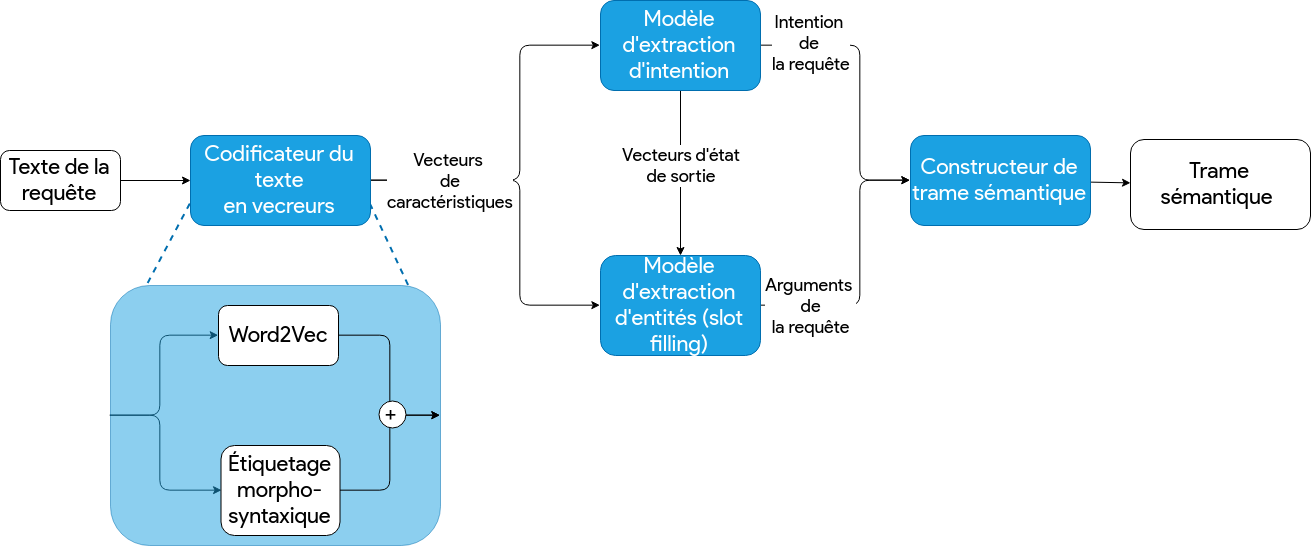
\includegraphics[width=0.88\linewidth]{images/Conception/NLU/nlu_module_arch.png}
		\caption{Architecture du module  compréhension automatique du langage naturel}
	\end{figure}
	\paragraph{}
	Comme précédemment cité (voir \ref{system_layer}), le module possède une architecture en pipeline qui reçoit en entrée le texte brut de la requête, sa codification varie selon les approches que nous avons exploré et qui seront plus expliciter dans le chapitre suivant Réalisation et Expérimentions, pour mieux capturer l'aspect sémantique des mots dans le texte, nous avons décidé d'utiliser un modèle pré-entraîné par Google de Word2Vec (entraîné sur 100 milliard de mots) pour produire un vecteur de taille fixe pour chaque mots, pour encoder l'information syntaxique de la requête nous avons concaténé au vecteur de prolongement de chaque mot de la requête (Word Embedding Vector) le vecteur codifiant son étiquette morphosyntaxique. Après avoir codifié la séquence de mots, elle est envoyée aux modèles de classification d'intentions et d'extraction d'entités \footnote{Par entité nous entendons les arguments de l'intention}, qui sont en fait un seul modèle joint dont l'architecture est détailler dans \ref{joint_model}. Ces deux informations sont ensuite décodées et passées au constructeur de trame sémantique qui structurera ces dernières en une seule entité sémantique dans le format suivant : 
	donnant le format suivant \begin{lstlisting}[language=json]
	{
		intent  : "open_file_desire",
		entities : [
			{	
				entity	: "string",
				name	: "file_name",
				value	: "tes.py",
				start	: "31",
				end		: "37",
			}
		]
	}
	\end{lstlisting}
	
%	\subsection{Analyse sémantique basée sur les grammaires de dépendances}
	\subsection{Analyse sémantique avec apprentissage automatique}
		\subsubsection{Modèle(s) utilisé}
		\paragraph{}\label{joint_model}
		Comme vu dans le chapitre précédent (voir \ref{nlu_chap2}) l'architecture adopté est une architecture mono-entrée/multi-sorties dont l'entrée est une séquence de mots codifiés et les sorties sont une séquence d'étiquettes et une classe associé au texte. Nous pouvons distingué les deux parties qui sont l'encodage et le décodage de la séquence, l'encodage sert à la fois à l'attribution de la classe (l'intention) et à l'initialisation de la séquence de décodage (pour l'attribution de son étiquette à chaque mot).
		\par
		L'encodage se fait en utilisant un réseau de neurones récurent de type BLSTM (Bidirectionnel Long Short Term Memory) pour mieux capturer le contexte droit (respectivement gauche) de chaque entrée, le dernier vecteur en sortie est ensuite utilisé comme vecteur d'entrée pour un réseau de neurones Fully Connected (Complètement connecté) dont la dernière couche est une couche de prédiction sur une distribution de probabilités des intentions possibles. Ce dernier vecteur sert aussi de d'état initial au décodeur qui est aussi un réseau de neurones récurent de type BLSTM, à chaque étape de l'inférence une étiquette est produite en sortie pour chaque position du texte en entrée (les longueur des séquences d'entrée et de sortie sont donc égales) en utilisant un autre réseau de neurone Fully Connected sur chaque vecteur d'état de sortie des cellules LSTM du décodeur (voir ~\ref{fig:lstmslots})
		\subsubsection{Les données d'apprentissage}
		\paragraph{}
		Ne disposant pas d'un ensemble d'apprentissage pré-existant pour les intentions que nous avons développé, nous avons tenté d'en construire un nous même en l'enrichissant avec quelque modifications. Dans \cite{rasa_nlu} il a été noté que pour une tâche assez simple (comme pour notre cas l'exploration des fichiers dans un premier temps) une grande quantité de données n'est pas nécessaire (une cinquantaine d'exemples par intentions approximativement) si les exemples ne sont pas facilement confondus, surtout si l'espace des possibilité pour les requête est assez réduit et peut facilement être expliciter. En jouant sur l'ordre des mots nous avons pu générer pour les XX intentions YYY patrons d'exemple au total (TOTAL PEUT ENCORE ÊTRE CHANGÉ 361 pour l'instant), un patron d'exemple une structure contenant des placeholders (compartiment) pouvant être rempli avec des valeurs généré programmatiquement, par exemple : 
		\begin{lstlisting}[language=json]
		delete the {file_name:} file under {parent_directory:}\end{lstlisting}
		Ces placeholders servent à la fois à générer plus d'exemples mais aussi à étiqueter le texte en chosifiant les valeurs de ces variables comme valeur de l'étiquette, un exemple d'un entrée de l'ensemble d'apprentissage avant affectation des variables est le suivant : 
		\begin{lstlisting}[language=json]
		
		{
			"id": 6,
			"text": "I want to open the {file_name:} folder",
			"intent": "open_file_desire"
		},
		\end{lstlisting}
		Pour remplir l'ensemble des placeholders, nous commençons d'abord par scanner le répertoire de la machine avec une profondeur max égale à 5,
		Les noms des répertoires sont donc nettoyé à l'aide d'expressions régulière et transformé en un format universel établi ç l'avance \textbf{nom\_du\_fichier} en choisissant "\_" comme séparateur, en bouclant sur ces noms de répertoire nous pourrons donc construire plusieurs exemples comme une entré dans un dictionnaire dont le format est le suivant : 
		\begin{lstlisting}[language=json]
		{
			'id': 79372,
			'intent': 'close_file_desire',
			'postags': ['NN', 'VB', 'DT', 'NN', 'VBN', 'NN', 'NNS'],
			'tags': 'NUL NUL NUL NUL NUL file_name file_name',
			'text': 'please close the file named platform notifications'
		}
		\end{lstlisting}
\section{Module de gestion du dialogue}
Le but de ce module est de décider quelle action à prendre à chaque instant du dialogue. D’abord nous allons présenter l’architecture globale de ce module notamment la représentation des informations reçues et la politique d’action. Ensuite, nous allons détailler la conception de chaque partie.
\subsection{Architecture du module}
Comme nous avons déjà vu, l’architecture typique des gestionnaires de dialogue se compose de deux parties principales: 
\begin{itemize}
	\item Un module qui suit l’état du dialogue : Pour gérer le dialogue avec l’utilisateur, le gestionnaire doit représenter l’état du dialogue de façon à pouvoir répondre aux actions de l’utilisateur. Ce module sert à suivre cet état après chaque étape du dialogue.
	\item Une politique d’action : Celle-ci détermine l’action à prendre à partir d’un état donné.
\end{itemize}
\subsubsection{État du dialogue}
Avant de détailler les deux modules du gestionnaire. Il est nécessaire d’introduire une représentation de l’état du dialogue. Classiquement, les trames sémantiques sont utilisés \ref{trame}. Le suivi d’état se fait dans ce cas en gardant trace des emplacements remplis durant le dialogue \ref{suivi}.
Nous avons opter à utiliser une représentation plus riche ; les graphes de connaissances sont une forme de représentation où les connaissances sont décrites sous forme d’un graphe orienté étiqueté. Des travaux ont déjà utilisé des graphes de connaissances\cite{Stoyanchev2018} et des ontologies\cite{Wessel2019} pour représenter l’état du système de dialogue. Celui-là est suivi d’une base de règles pour décider l’action à prendre directement du graphe de connaissances. L’avantage par rapport à l’utilisation des trames sémantiques apparaît dans la flexibilité et le dynamisme des graphes de connaissances. En effet, pour une tâche comme la navigation dans les fichiers, l’état de l’arborescence des fichiers est sujet à des changements fréquents : ajout, suppression, modification, etc. Il est difficile de faire une représentation de l’information dans ce cas avec de simples emplacements à remplir.
\subsubsection{Le suivi de l’état du dialogue}
Le rôle du premier module est de mettre à jour l’état du système au cours du dialogue. Il reçoit l’action de l’utilisateur ou du gestionnaire et il produit un nouvel état comme le montre la figure\ref{tracker1}.
\begin{figure}[H] 
	
	\centering
	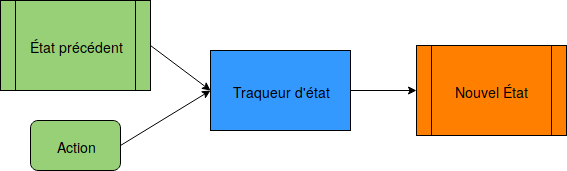
\includegraphics[width=0.88\linewidth]{images/Conception/DM/Tracker1.png}
	\caption{Schéma du traqueur d'état}
\end{figure}\label{tracker1}
\paragraph{}
Dans notre cas, le module NLU produit toujours un trame sémantique à partir du texte contenant l’intention de l’utilisateur ainsi que ses paramètres. C’est alors le travail du traqueur d’état d’injecter le résultat du NLU dans le graphe de connaissances. Ceci consiste à transformer le trame sémantique en un graphe selon des règles de transformation qui est ensuite ajouté au graphe d’état. Plus de détails seront donnés dans la section suivante\ref{onto} où nous construirons une ontologie pour définir un vocabulaire de dialogue et comment elle peut être utilisé pour passer du résultat du NLU en un graphe de connaissances.
\begin{figure}[H] 
	
	\centering
	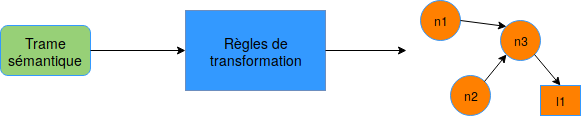
\includegraphics[width=0.88\linewidth]{images/Conception/DM/Transformer.png}
	\caption{Schéma de transformation de trame sémqntique en graphe}
\end{figure}\label{transformer}
\subsubsection{La politique d’action}
La politique d’action peut être écrite manuellement ou apprise à partir d’un corpus ou en utilisant l’apprentissage par renforcement. Dans ce dernier cas, un agent doit interagir avec un utilisateur qui évalue ses performances afin qu’il puisse apprendre. Étant donné que l’apprentissage par renforcement nécessite un nombre important d’interactions, il est primordial d’utiliser un simulateur d’utilisateur. Ce dernier peut être basé règles, ou un modèle statistique extrait à partir d’un corpus de dialogue.\\
Dans les trois cas de figure, il est difficile de réaliser un modèle varié et qui peut accomplir plusieurs tâches. D’un coté, un corpus contenant des dialogues sur toutes les tâches possibles, si ces derniers sont nombreux et spécifiques à une application précise, est difficile à acquérir. De l’autre coté, écrire les règles d’un système de dialogue ou d’un simulateur d’utilisateur s’avère compliqué et nécessite un travail manuel énorme pour gérer toutes les tâches possibles.\\
Pour pallier à cela, nous proposons d’utiliser une architecture multi-agents hiérarchique. Dans laquelle, les agents feuilles sont des agents qui peuvent répondre à une tâche ou une sous tâche bien précise. Tandis que les agents parents sélectionnent l’agent fils capable de répondre à l’intention de l’utilisateur.
\begin{figure}[H] 
	
	\centering
	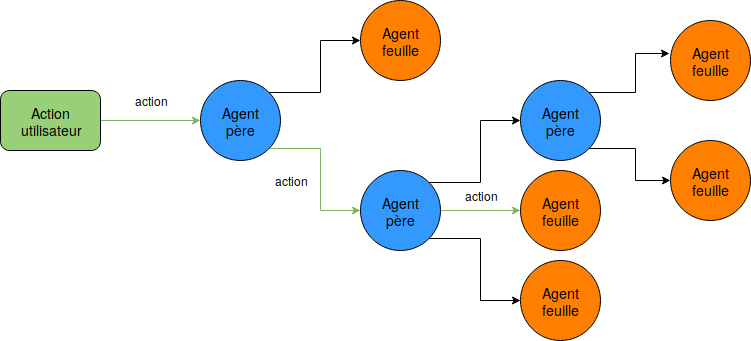
\includegraphics[width=0.88\linewidth]{images/Conception/DM/multiagent.png}
	\caption{Schéma de l'architecture multi-agents}
\end{figure}\label{multiagent}
L’avantage d’une telle architecture est de permettre la division du problème en plusieurs sous problèmes indépendants. En effet, un simulateur d’utilisateur ou un corpus qui est destiné pour une seule tâche est considérablement plus abordable.  Cependant, un travail supplémentaire s’avère nécessaire qui est celui des agents parents. Celui-ci est relativement simple, il suffit de faire un apprentissage supervisé des agents parents avec les simulateurs d’utilisateurs des agents fils. à tour de rôle et avec des probabilités de transitions entre les simulateurs d’utilisateurs, ces derniers communique avec l’agent parent. Comme on connaît pour chaque simulateur l’agent fils qui lui correspond, il est donc possible de faire un apprentissage supervisé où les entrées sont les actions des simulateurs et l’état du système, tandis que la sortie est l’agent fils qui peut répondre à l’action.
\begin{figure}[H] 
	
	\centering
	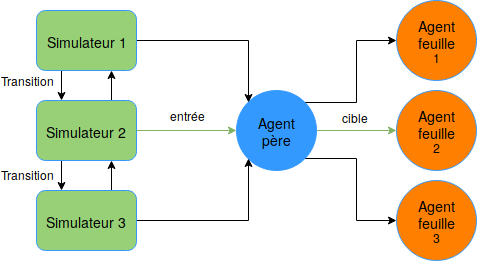
\includegraphics[width=0.7\linewidth]{images/Conception/DM/train_parent.png}
	\caption{Schéma représentant l'apprentissage des agents parents avec les simulateurs des agents feuilles}
\end{figure}\label{train_parent}
\paragraph{}
Pour résumer l’architecture globale du gestionnaire de dialogue, lorsque une nouvelle action utilisateur arrive au système, le traqueur d’état la reçoit. Il met à jour l’état du système en transformant l’action en un graphe de connaissances pour l’ajouter au graphe d’état. Ce nouvel graphe d’état ainsi que la dernière action reçue sont transmis à une architecture multi-agents hiérarchique qui va décider quelle action le système de dialogue doit prendre.
\begin{figure}[H] 
	
	\centering
	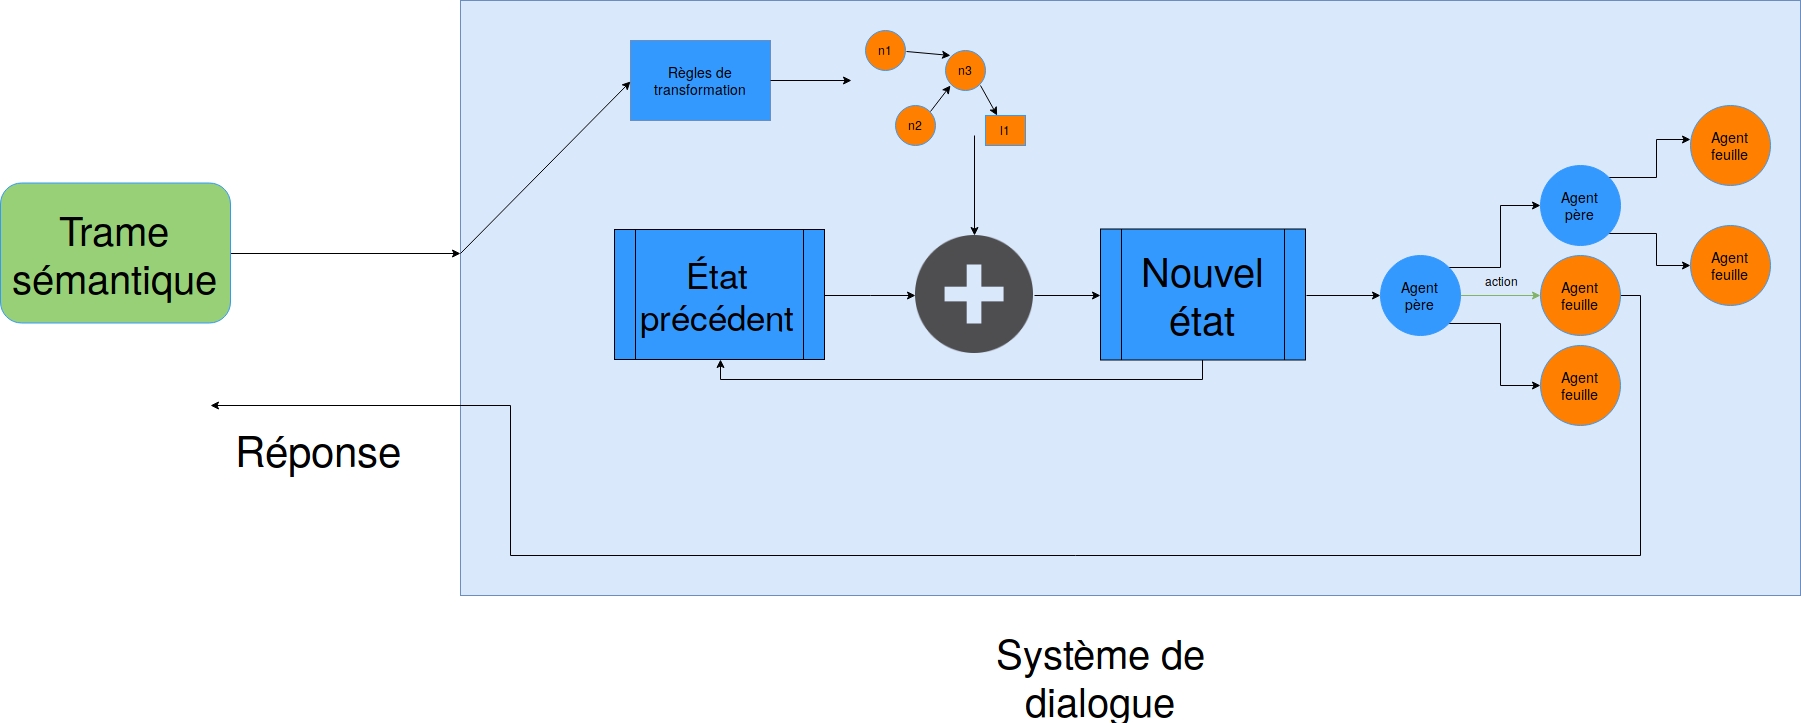
\includegraphics[width=0.88\linewidth]{images/Conception/DM/globalDM.png}
	\caption{Schéma global du gestionnaire de dialogue}
\end{figure}\label{globalDM}
	\subsection{Les ontologies du système}\label{onto}
		Une ontologie est une représentation des concepts et les relations d’un domaine donné, elle permet de définir un vocabulaire pour ce domaine afin que les programmes intelligents puissent comprendre  et communiquer sur des données reliées à ce domaine.\\
		Nous définissons une ontologie de dialogue ainsi que des ontologies pour chaque tâche réalisable par notre assistant. Ce qui permettra à notre gestionnaire de comprendre le dialogue et les tâches qu’il peut réaliser.
		\subsubsection{Ontologie de dialogue}
		D’abord on définit une ontologie de dialogue qui contient des concepts qui peuvent aider un assistant d’ordinateur pour gérer son dialogue.
		FIGURE TOOODOOOOOOO
		Principalement l’ontologie se compose de six classes mères:
		\begin{itemize}
			\item $Agent$ et$ User$ : ce sont les classes qui représentent l’utilisateur et l’agent qui participent au dialogue.
			\item $Dialogue$ : l’agent et l’utilisateur participe à un dialogue, ce dernier contient les actions des deux cotés.
			\item $Dialogue\_act$ : la classe qui représente une action du dialogue, elle a deux sous-classes $Agent\_act$ et $User\_act$ qui représentent les actions de l’agent et de l’utilisateur respectivement.
			\item $Act\_parameter$ : C’est la classe mère des paramètres que peuvent prendre les actions de dialogue. Par exemple, l’action d’informer peut avoir en paramètre le nom d’un fichier.
			\item $Act\_desire$ : C’est la classe mère des actions de l’agent que l’utilisateur peut demander. Par exemple, il peut demander l’ouverture d’un fichier donné.
		\end{itemize}
	Le reste des classes sont des classes filles qui détaillent plus les concepts du dialogue agent-utilisateur.\\
	À l’arriver d’une nouvelle action, le traqueur d’état va créer le graphe correspondant. Un exemple abstrait de cela est représenté dans la figure \ref{abstract_onto}. Une nouvelle action utilisateur est créer ainsi que ses paramètres et les relations entre eux.
	\begin{figure}[H] 
		\centering
		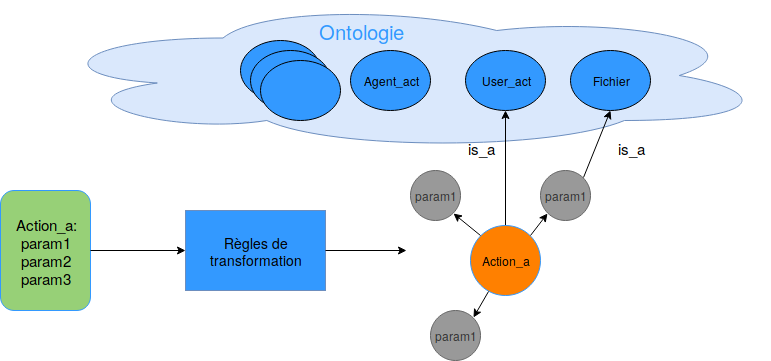
\includegraphics[width=0.88\linewidth]{images/Conception/DM/abstract_onto.png}
		\caption{Schéma de transformation d'une action en graphe}
		
	\end{figure}\label{abstract_onto}
		\subsubsection*{Ontologie pour l’exploration de fichiers}
		Un exemple d’ontologie pour la compréhension d’une tâche réalisable par l’assistant est celle de l’exploration de fichiers.
		FIGURE TOOODOOOOOO
		L’ontologie contient essentiellement :
		\begin{itemize}
			\item Des actions sur les fichiers : Créer un fichier, supprimer un fichier, changer de répertoire, etc. Ces actions sont des sous-classes de la classe  $Agent\_act$ vu précédemment ainsi que les classes $Act\_parameter$ et $Act\_desire$. Ce qui veut dire que ces actions peuvent être des paramètres d’autres actions comme demander à l’utilisateur s’il veut que l’assistant réalise une action donné et que l’utilisateur peut demander à l’assistant de faire une de ces actions. 
			\item Les concepts qui ont relation avec l’exploration de fichiers sont des sous-classes de $Act\_parameter$ étant donné qu’ils peuvent  être des paramètres d’actions, par exemple l’action d’ouvrir un fichier a comme paramètre un fichier.
			\item Des relations entre ces concepts sont aussi définies comme un répertoire peut contenir des fichiers, ou une action de changement de répertoire doit avoir comme paramètre un répertoire cible.
		\end{itemize}
	La figure suivante \ref{nonabstract_onto} représente l’arrivé d’une nouvelle action : « créer un fichier nommé ‘travail’ ». l’action de l’utilisateur est donc représentée par un nouveau nœud de type $U\_act\_desire$ qui désigne une action utilisateur qui demande une action de l’assistant. Cette dernière a comme paramètre un nœud de type $Create_file$ qui est l’action de l’agent que l’utilisateur veut réaliser. Cette action à son tour a des paramètres comme, dans ce cas, le fichier qu’on veut créer.
	\begin{figure}[H] 
		\centering
		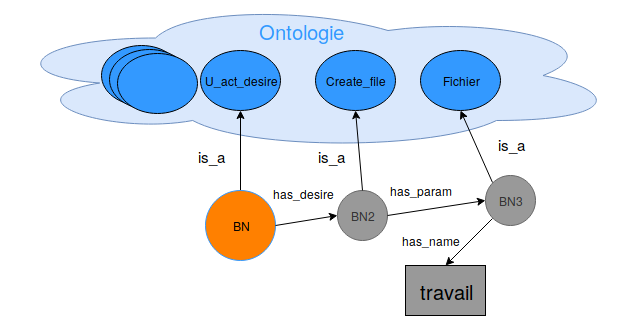
\includegraphics[width=0.88\linewidth]{images/Conception/DM/nonabstract_onto.png}
		\caption{Schéma de transformation d'une action de demande de création de fichier en graphe}
		
	\end{figure}\label{nonabstract_onto}
Les autres actions sont créer de façon similaire avec des règles à suivre lorsqu’une nouvelle action arrive.
	\subsection{Les simulateurs d'utilisateurs}
	Plusieurs méthodes peuvent être utilisés pour la création de simulateurs d’utilisateurs\ref{usersim}. Les simulateurs basés sur des méthodes d’apprentissage sont les plus robustes. Cependant, ils nécessitent un nombre important de données. L’alternative c’est d’utiliser des simulateurs basés règles. Nous nous sommes inspirés des simulateurs basés agenda\cite{Schatzmann2007} qui sont des variantes des simulateurs basés règles pour créer nos propres simulateurs. Leur fonctionnement est simple, Ils commencent par générer un but. Pour y arriver, une agenda est créée, celle-ci contient les informations que doit convoyer le simulateur ainsi que les informations qu’il doit recevoir. Les actions sont sélectionnées en suivant des probabilités conditionnelles sur l’état de l’agenda. Enfin, les récompenses sont en fonction des informations reçues de l’agent.
	\subsubsection*{Simulateur pour l’exploration de fichiers}
	L’exploration de fichiers ne dépend pas de simples informations à transmettre et d’autres à recevoir comme dans les cas d’envoyer un e-mail, chercher une information sur internet ou bien lancer de la musique. Il s’agit d’une tâche dynamique dont la situation de départ est variante. Pareillement, le nombres d’actions change d’un état à un autre. Effectivement, le nombre de fichiers qu’on peut supprimer ou le nombre de répertoires qu’on peut y accéder n’est pas fixe par exemple.
	D’abord une arborescence aléatoire est générée qui représente la situation initiale du système. Ensuite, le simulateur duplique cette arborescence en y introduisant des modifications pour générer une arborescence but. Enfin, le simulateur essaye de guider l’agent pour arriver au but en utilisant les actions utilisateurs possibles.\\
	En addition des actions de création et suppression de fichiers ainsi que les changements de répertoires qui peuvent guider l’agent au but. D’autres sous-buts peuvent être créés suivant une distribution de probabilité comme copier ou couper un fichier, renommer un fichier, ouvrir un fichier etc. Dans ce cas le simulateur donne la priorité aux sous-buts avant de reprendre les actions menant au but final.\\
	L’algorithme suivi par le simulateur est le suivant :
	ALGOOOOOOOOOTODOOOOOOOOOO\\
	Quant à la décision de l’action à prendre, elle est résumée par le diagramme suivant :
	\begin{figure}[H] 
		\centering
		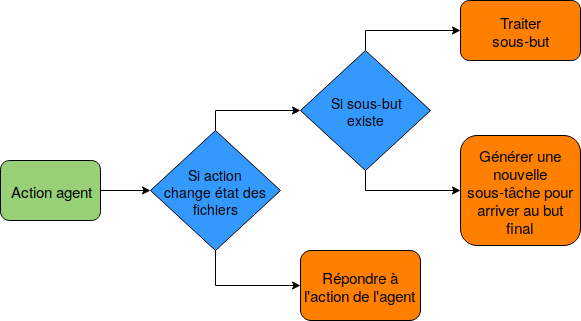
\includegraphics[width=0.8\linewidth]{images/Conception/DM/action_diag.png}
		\caption{Diagramme de décision de l'action à prendre}
		
	\end{figure}\label{action_diag}
En ce qui concerne la fonction de récompense, celle-ci est évaluée à partir des changements effectués sur l’état de l’utilisateur, le tableau suivant \ref{table_reward} associe les changements avec leurs récompenses :
\begin{table}[H]\label{table_reward}
	\begin{center}
		
		\begin{tabular}{l|c} % <-- Alignments: 1st column left, 2nd middle and 3rd right, with vertical lines in between
			\textbf{Événements} & \textbf{Récompenses}\\
			\hline
			Similarité améliorée & 2\\
			\hline
			Succès & 2\\
			\hline
			Sous-but réalisé & 2\\
			\hline
			Similarité diminuée & -3\\
			\hline
			Confirmation d'une question & 0\\
			\hline
			Autre & -1\\
			\hline
		\end{tabular}
	\caption{Tableau des récompenses}
	\end{center}
\end{table}
\begin{itemize}
	\item \textbf{similarité améliorée:} On calcule la similarité entre l'arborescence courante et l'arborescence but. La valeur de la similarité est égale à $n\_sim/n\_diff$ avec : 
	\begin{itemize}
		\item $n\_sim$ : nombre de fichiers qui existent dans les deux arborescences.
		\item $n\_diff$ : nombre de fichiers qui n’existent que dans une des deux arborescences.  
	\end{itemize}
	\item \textbf{Succès:} c'est à dire, réaliser le but final du simulateur. Pour arriver à cet événement, l'agent ne fait qu'améliorer la similarité, c'est pourquoi les deux événements ont la même valeur de récompense.
	\item \textbf{Sous-but réalisé:} c'est la récompense donnée quand l'agent arrive au sous-but du simulateur.
	\item \textbf{Similarité diminuée:} la récompense est dans ce cas négative et supérieur en valeur absolue à celle que l'agent obtient lorsqu'il améliore la similarité. Ce choix a pour but d'éviter que l'agent boucle sur des actions dont la somme des récompenses est supérieur ou égale à zero. Par exemple il peut créer ensuite supprimer le même fichier, si la somme de ces deux actions est supérieur ou égale à zéro, l'agent peut boucler sur ces actions indéfiniment sans pour autant recevoir des récompenses négatives.
	\item \textbf{Confirmation d'une question:} l'utilisateur peut confirmer une action à l'agent. La récompense est nul pour que l'agent puisse demander une confirmation quand il n'est pas sûr de ce qu'il doit faire sans diminuer le cumule des récompenses reçues.
	\item \textbf{Autre:} La récompense est de -1 pour éviter que le dialogue dure long temps. 
\end{itemize}
Pour résumer le fonctionnement du simulateur, à l’arrivé d’une nouvelle action agent, celle-ci met à jour l’état du simulateur. L’état du simulateur se compose de deux parties : un simulateur d’arborescence de fichiers qui simule l’état de l’arborescence courant, et des variables d’état qui contiennent d’autres informations comme l’état des sous-buts, le fichier en cours de traitement, les informations reçues de l’agent, le répertoire courant, etc. Après la mise à jour de l’état, si l’action de l’agent nécessite une réponse immédiate comme la demande d’une information ou la permission d’exécuter une action, celle-ci est traité directement, sinon le simulateur initie le traitement d’une nouvelle sous-tâche. C’est à dire, Si un sous-but existe, une action qui le traite est générée, sinon une action qui traite le but final est générée.
	\subsection{Modèles d'apprentissage}
	Comme on l’a déjà cité dans le chapitre précédent, il existe plusieurs algorithmes d’apprentissage par renforcement comme Q-Learning ou State-Action-Reward-State-Action (SARSA)\cite{Rummery1994}. Cependant ces algorithmes, en essayant d’estimer la fonction Q de récompense, traitent le problème comme un tableau état/action et essayent d’estimer pour chaque état et action la récompense résultante. Ceci implique que ces algorithmes ne peuvent pas estimer la fonction de récompense pour des état qu’ils n’ont pas vu pendant l’apprentissage. Pour pallier à ce problème, Deep Q Learning (DQL)\cite{Mnih2015} utilise un réseau de neurones comme estimateur de la fonction Q. Ce qui lui permet d’avoir une notion de similarité entre les états ; ainsi il peut estimer la récompense pour des états jamais vus auparavant.
	\subsubsection*{Encodeur de graphe}
	La flexibilité des graphes les rend difficile à introduire dans un réseau de neurones vu que ce dernier n’accepte que des entrées de tailles fixes. Des méthodes ont été utilisées pour introduire les graphes dans des réseaux de neurones notamment les convolutions sur les graphes avec Graph Convolution Networks (GCN)\cite{KipfW17} qui s’avère être des variantes des Gated Graph Neural Networks (GGNN)\cite{Li2016GatedGS}. Ce dernier utilise des réseaux de neurones récurrent entre chaque deux nœuds reliés par une arrête pour transférer l’information d’un nœud à un autre, ce qui résulte en des vecteurs ayant un encodage de l’information associé à chaque nœud. Cette étape est répétée k fois pour que chaque nœud aie des informations des nœuds qui sont à un maximum de k pas de distance, avec k un paramètre empirique. Enfin, les vecteurs d’états de chaque nœud sont sommés pour produire un vecteur fixe encodant tout le graphe qui peut être relié au reste du réseau de neurones pour l’apprentissage.
	\begin{figure}[H] 
		\centering
		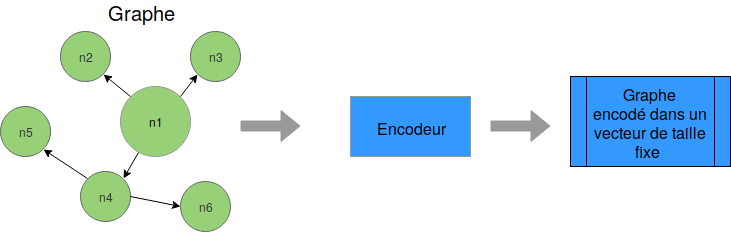
\includegraphics[width=0.8\linewidth]{images/Conception/DM/encoder.png}
		\caption{Schéma représentant un encodeur de graphe}
		
	\end{figure}\label{encoder}
Ces méthodes nécessitent tout le graphe pour l’encoder. Cependant, dans notre cas, après chaque action, le graphe augmente de taille ce qui nécessite de refaire l’encodage dès le début. Nous proposons de traiter le graphe comme une séquence de triplets: « nœud ; arc ; nœud » ou « sujet ; predicat ; objet » comme dans le framework Resource Description Framework (RDF). L’encodage se fait avec une architecture encodeur-décodeur basé sur des réseaux de neurones récurrent (RNN). Ainsi, à l’arriver de nouveaux triplets, il suffit d’utiliser l’état précédent pour y encoder les nouveaux triplets.
\begin{figure}[H] 
	\centering
	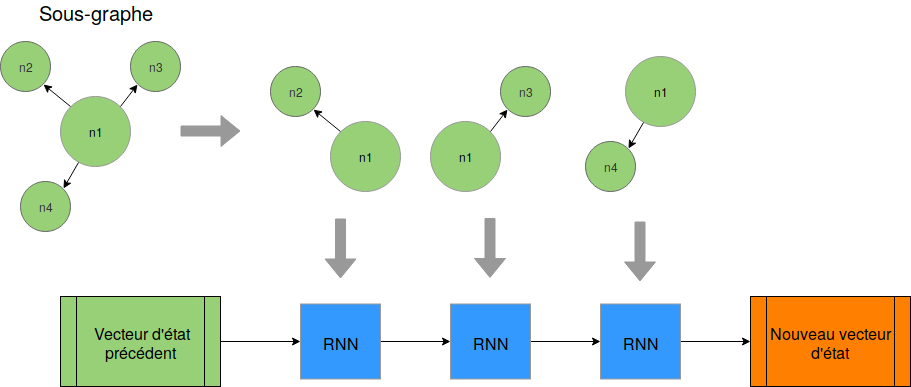
\includegraphics[width=0.8\linewidth]{images/Conception/DM/encoder_seq.png}
	\caption{Schéma représentant un encodeur séquentiel de graphe}
	
\end{figure}\label{encoder_seq}
Pour faire l’apprentissage de cet architecture, il est possible de générer des graphes aléatoirement qu’on fait passer triplet par triplet dans l’encodeur. Celui-ci est un RNN qui prend en entrée l’état précédent du réseau et un triplet du graphe et qui produit en sortie un nouvel état. L’état final du RNN, après avoir fait passer tous les triplets du graphe, est utilisé dans le décodeur qui est un autre RNN. Ce dernier essaye de reconstruire le graphe triplet par triplet à partir de l’état reçu comme sortie de l’encodeur. Ainsi, si on peut reconstruire le graphe, on peut dire que le dernier état encode tout le graphe dans un vecteur de taille fixe.
\begin{figure}[H] 
	\centering
	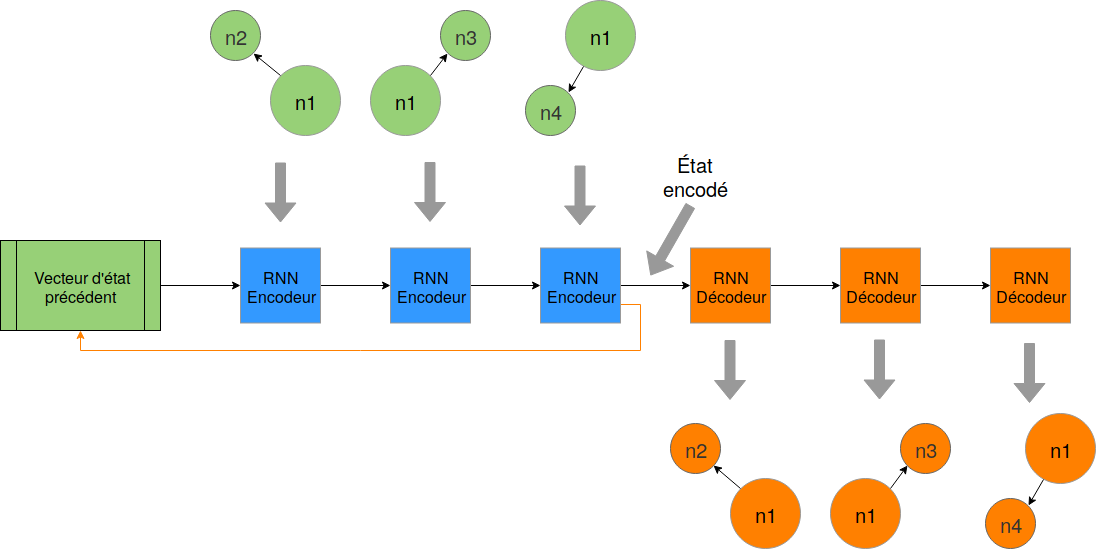
\includegraphics[width=0.8\linewidth]{images/Conception/DM/encoder_seq_train.png}
	\caption{Schéma de l'apprentissage d'un encodeur séquentiel de graphe}
	
\end{figure}\label{encoder_seq_train}
\subsubsection*{Les agents feuilles}
Comme nous en avons parlé précédemment, les agents feuilles sont les agents responsable de répondre aux intentions de l’utilisateur. Pour faire l’apprentissage par renforcement d’un agent feuille, on utilise le simulateur d’utilisateur comme environnement de cet agent. Ce dernier interagit avec le simulateur pour but d’estimer la fonction de récompense en fonction de son état. On utilise pour cela un réseau de neurones profond qui prend en entrée l’état encodé de l’agent, c’est à dire le graphe encodé, et il produit pour chaque action la récompense correspondante. Comme le nombre d’actions est variable, il est impossible d’utiliser une architecture de réseau de neurones qui produit une sortie pour chaque action, où chaque sortie est la récompense de l’action qui y correspond. Par conséquent, il est nécessaire de donner au réseau, en addition de l’état encodé, l’action candidate.
\begin{figure}[H] 
	\centering
	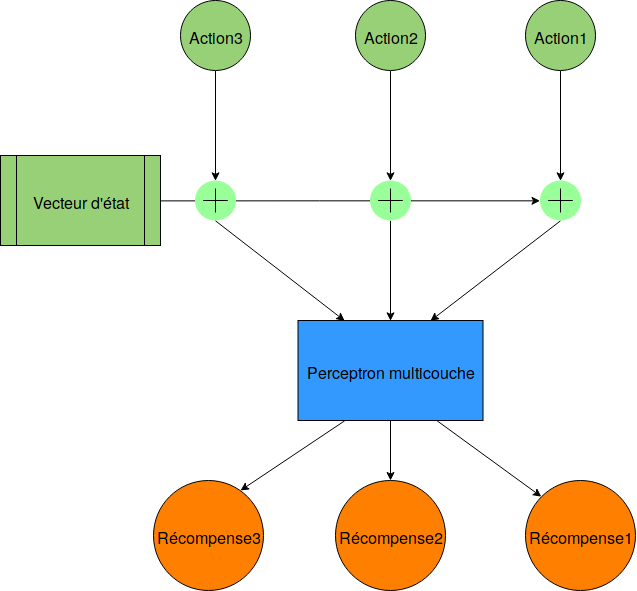
\includegraphics[width=0.7\linewidth]{images/Conception/DM/time_dist.png}
	\caption{Schéma du réseau DQN}
\end{figure}\label{time_dist}
L’algorithme utilisé pour l’apprentissage par renforcement est double DQN en rejouant l’expérience. En addition de l’utilisation des réseaux de neurones pour estimer la fonction Q, deux amélioration lui ont été ajoutées :
\begin{itemize}
	\item rejouer l’expérience : l’agent interagit avec le simulateur plusieurs fois en gardant dans une mémoire ses interactions. Après chaque k épisode\footnote{un épisode est un ensemble d’interactions agent-simulateur jusqu’à finir avec un succès ou échec} l’agent reprend la mémoire pour entraîner le réseau de neurones.
	\item Double DQN : la fonction Q est donné par la formule $Q(s,a) = r + \alpha*max_j(Q(s’,a_j))$ avec :
	\begin{itemize}
		\item $s$ : état de l’agent.
		\item $a$ : l’action qu’on veut estimer.
		\item $R$ : récompense immédiate.
		\item $\alpha$ : paramétré de réduction.
		\item $s’$ : nouvel état après avoir effectuer l’action a de l’état $s$.
		\item $a_j$ : les actions possibles à partir de l’état s’.
	\end{itemize}
On remarque la récurrence dans cette formule qui nécessite la réutilisation du réseau pour estimer le terme $max_j (Q(s’,a_j))$. Il a été démontré que l’utilisation d’un autre réseau qu’on fixe lors de l’apprentissage pour l’évaluation de la récompense dans ce terme améliore les résultats\cite{Mnih2015}. La formule devient donc : $Q(s,a) = r + \alpha*Q(s’,argmax_{a_j}(s’,a_j))$. Cette valeur est donc utilisé pour calculer l’erreur et appliquer l’algorithme de retro-propagation pour l’apprentissage automatique.
\end{itemize}
Une autre architecture possible serait de relier l’encodeur de graphe directement avec le réseau DQN pendant l’apprentissage. Ainsi l’erreur de l’apprentissage pour l’encodeur est calculer à partir de la fonction de récompense de l’apprentissage par renforcement. L’avantage de relier l’encodeur avec le réseau de DQN est de permettre à l’encodeur de contrôler quelle partie du graphe encodé à oublié. En effet, la taille fixe du vecteur dont on encode le graphe a une limite de nombre de triplets supportable. L’utilisation des cellules de réseaux de neurones récurrent comme les LSTMs ou GRUs qui ont des porte d’oublie rend cette architecture possible.
\begin{figure}[H] 
	\centering
	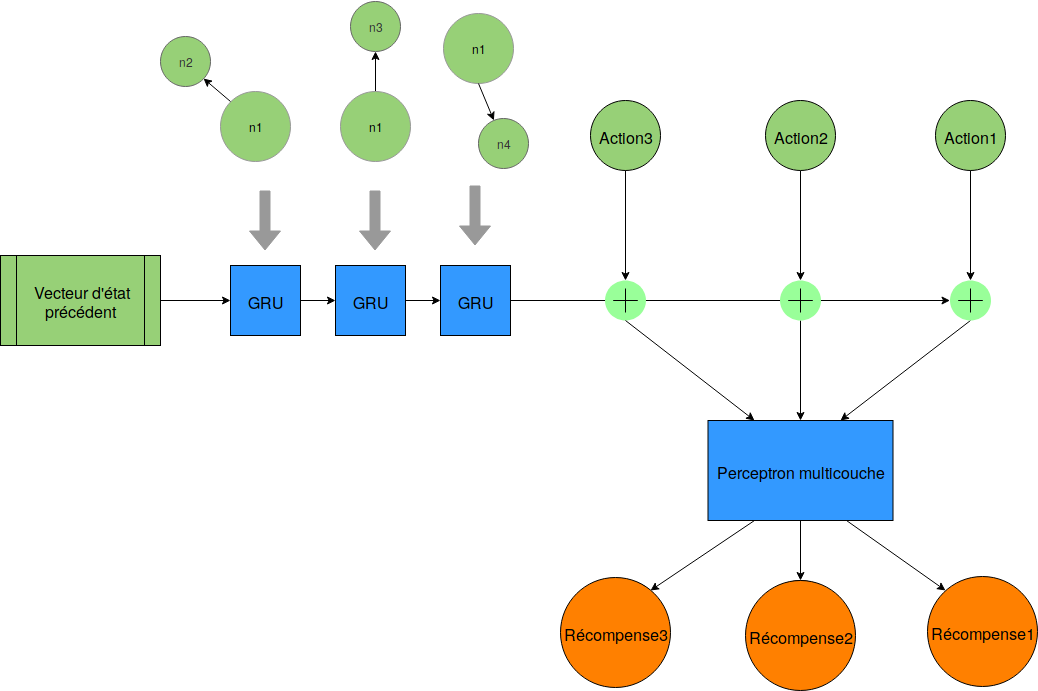
\includegraphics[width=0.88\linewidth]{images/Conception/DM/encoder_dqn.png}
	\caption{Schéma du réseau DQN relié avec l'encodeur directement}
\end{figure}\label{encoder_dqn}
\subsubsection*{L'agent coordinateur}
L’agent coordinateur utilise la même architecture que celle des agents feuilles. La différence se trouve au niveau de la sortie. Dans le cas des agents coordinateurs, ils essayent de prédire quelle agent fils peut répondre à la dernière action reçue.
\section{Module de génération du langage naturel}
Le modèle utilisé pour la génération du texte est relativement simple. Il s’agit de préparer des modèles de phrases contenant des emplacements à remplir. Chaque action de l’agent lui correspond un ensemble de modèles et chaque paramètre de l’action lui correspond un ensemble d’expressions. La génération du texte se fait en choisissant d’abord pour chaque paramètre de l’action une expression aléatoirement. Ensuite, de même, un modèle de phrase est choisit aléatoirement. Enfin, les emplacements vides sont remplis avec les expressions des paramètres. La figure suivante illustre un exemple de la génération de texte en utilisant les modèles de phrases.
\begin{figure}[H] 
	\centering
	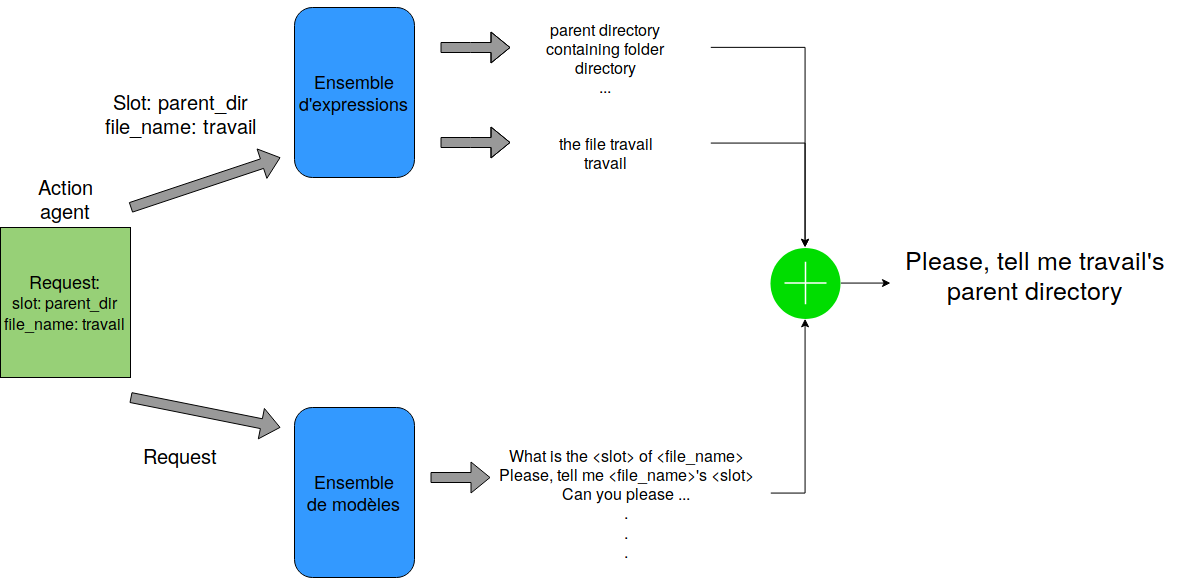
\includegraphics[width=0.95\linewidth]{images/Conception/NLG.png}
	\caption{Schéma de fonctionnement du générateur de texte}
\end{figure}\label{nlg_schema}
\section{Conclusion}
 %%%%%%%%%%%%%%%%%%%%%%%%%%%%%%%%%%%%%%%%%%%%%%%%%%%%%%%%%%%%%%%%%%%%
%        Generated with the experimental alpha version of the TeX exporter of WebVOWL (version 1.1.3) %%% 
%%%%%%%%%%%%%%%%%%%%%%%%%%%%%%%%%%%%%%%%%%%%%%%%%%%%%%%%%%%%%%%%%%%%

%   The content can be used as import in other TeX documents. 
%   Parent document has to use the following packages   
%   \usepackage{tikz}  
%   \usepackage{helvet}  
%   \usetikzlibrary{decorations.markings,decorations.shapes,decorations,arrows,automata,backgrounds,petri,shapes.geometric}  
%   \usepackage{xcolor}  

%%%%%%%%%%%%%%% Example Parent Document %%%%%%%%%%%%%%%%%%%%%%%
%\documentclass{article} 
%\usepackage{tikz} 
%\usepackage{helvet} 
%\usetikzlibrary{decorations.markings,decorations.shapes,decorations,arrows,automata,backgrounds,petri,shapes.geometric} 
%\usepackage{xcolor} 

%\begin{document} 
%\section{Example} 
%  This is an example. 
%  \begin{figure} 
%    \input{<THIS_FILE_NAME>} % << tex file name for the graph 
%    \caption{A generated graph with TKIZ using alpha version of the TeX exporter of WebVOWL (version 1.1.3) } 
%  \end{figure} 
%\end{document} 
%%%%%%%%%%%%%%%%%%%%%%%%%%%%%%%%%%%%%%%%%%%%%%%%%%%%%%%%%%%%%%%%%%%%

\begin{figure}[H]
	 %%%%%%%%%%%%%%%%%%%%%%%%%%%%%%%%%%%%%%%%%%%%%%%%%%%%%%%%%%%%%%%%%%%%
 %        Generated with the experimental alpha version of the TeX exporter of WebVOWL (version 1.1.3) %%% 
 %%%%%%%%%%%%%%%%%%%%%%%%%%%%%%%%%%%%%%%%%%%%%%%%%%%%%%%%%%%%%%%%%%%%

 %   The content can be used as import in other TeX documents. 
 %   Parent document has to use the following packages   
 %   \usepackage{tikz}  
 %   \usepackage{helvet}  
 %   \usetikzlibrary{decorations.markings,decorations.shapes,decorations,arrows,automata,backgrounds,petri,shapes.geometric}  
 %   \usepackage{xcolor}  

 %%%%%%%%%%%%%%% Example Parent Document %%%%%%%%%%%%%%%%%%%%%%%
 %\documentclass{article} 
 %\usepackage{tikz} 
 %\usepackage{helvet} 
 %\usetikzlibrary{decorations.markings,decorations.shapes,decorations,arrows,automata,backgrounds,petri,shapes.geometric} 
 %\usepackage{xcolor} 

 %\begin{document} 
 %\section{Example} 
 %  This is an example. 
 %  \begin{figure} 
 %    \input{<THIS_FILE_NAME>} % << tex file name for the graph 
 %    \caption{A generated graph with TKIZ using alpha version of the TeX exporter of WebVOWL (version 1.1.3) } 
 %  \end{figure} 
 %\end{document} 
 %%%%%%%%%%%%%%%%%%%%%%%%%%%%%%%%%%%%%%%%%%%%%%%%%%%%%%%%%%%%%%%%%%%%

\definecolor{imageBGCOLOR}{HTML}{FFFFFF} 
\definecolor{owlClassColor}{HTML}{AACCFF}
\definecolor{owlObjectPropertyColor}{HTML}{AACCFF}
\definecolor{owlExternalClassColor}{HTML}{AACCFF}
\definecolor{owlDatatypePropertyColor}{HTML}{99CC66}
\definecolor{owlDatatypeColor}{HTML}{FFCC33}
\definecolor{owlThingColor}{HTML}{FFFFFF}
\definecolor{valuesFrom}{HTML}{6699CC}
\definecolor{rdfPropertyColor}{HTML}{CC99CC}
\definecolor{unionColor}{HTML}{6699cc}
\begin{center} 
\resizebox{\linewidth}{!}{
\begin{tikzpicture}[framed]
\clip (91.50651825285176pt , 101.92110741178745pt ) rectangle (1149.0692956695593pt , -743.5780149501337pt);
\tikzstyle{dashed}=[dash pattern=on 4pt off 4pt] 
\tikzstyle{dotted}=[dash pattern=on 2pt off 2pt] 
\fontfamily{sans-serif}{\fontsize{12}{12}\selectfont}
 
\tikzset{triangleBlack/.style = {fill=black, draw=black, line width=1pt,scale=0.7,regular polygon, regular polygon sides=3} }
\tikzset{triangleWhite/.style = {fill=white, draw=black, line width=1pt,scale=0.7,regular polygon, regular polygon sides=3} }
\tikzset{triangleBlue/.style  = {fill=valuesFrom, draw=valuesFrom, line width=1pt,scale=0.7,regular polygon, regular polygon sides=3} }
\tikzset{Diamond/.style = {fill=white, draw=black, line width=2pt,scale=1.2,regular polygon, regular polygon sides=4} }
\tikzset{Literal/.style={rectangle,align=center,
font={\fontsize{12pt}{12}\selectfont \sffamily },
black, draw=black, dashed, line width=1pt, fill=owlDatatypeColor, minimum width=80pt,
minimum height = 20pt}}

\tikzset{Datatype/.style={rectangle,align=center,
font={\fontsize{12pt}{12}\selectfont \sffamily },
black, draw=black, line width=1pt, fill=owlDatatypeColor, minimum width=80pt,
minimum height = 20pt}}

\tikzset{owlClass/.style={circle, inner sep=0mm,align=center, 
font={\fontsize{12pt}{12}\selectfont \sffamily },
black, draw=black, line width=1pt, fill=owlClassColor, minimum size=101pt}}

\tikzset{anonymousClass/.style={circle, inner sep=0mm,align=center, 
font={\fontsize{12pt}{12}\selectfont \sffamily },
black, dashed, draw=black, line width=1pt, fill=owlClassColor, minimum size=101pt}}

\tikzset{owlThing/.style={circle, inner sep=0mm,align=center,
font={\fontsize{12pt}{12}\selectfont \sffamily },
black, dashed, draw=black, line width=1pt, fill=owlThingColor, minimum size=62pt}}

\tikzset{owlObjectProperty/.style={rectangle,align=center,
inner sep=0mm,
font={\fontsize{12pt}{12}\selectfont \sffamily },
fill=owlObjectPropertyColor, minimum width=80pt,
minimum height = 25pt}}

\tikzset{rdfProperty/.style={rectangle,align=center,
inner sep=0mm,
font={\fontsize{12pt}{12}\selectfont \sffamily },
fill=rdfPropertyColor, minimum width=80pt,
minimum height = 25pt}}

\tikzset{owlDatatypeProperty/.style={rectangle,align=center,
fill=owlDatatypePropertyColor, minimum width=80pt,
inner sep=0mm,
font={\fontsize{12pt}{12}\selectfont \sffamily },
minimum height = 25pt}}

\tikzset{rdfsSubClassOf/.style={rectangle,align=center,
font={\fontsize{12pt}{12}\selectfont \sffamily },
inner sep=0mm,
fill=imageBGCOLOR, minimum width=80pt,
minimum height = 25pt}}

\tikzset{unionOf/.style={circle, inner sep=0mm,align=center,
font={\fontsize{12pt}{12}\selectfont \sffamily },
black, draw=black, line width=1pt, fill=unionColor, minimum size=25pt}}

\tikzset{disjointWith/.style={circle, inner sep=0mm,align=center,
font={\fontsize{12pt}{12}\selectfont \sffamily },
black, draw=black, line width=1pt, fill=unionColor, minimum size=20pt}}

\tikzset{owlEquivalentClass/.style={circle,align=center,
font={\fontsize{12pt}{12}\selectfont \sffamily },
inner sep=0mm,
black, solid, draw=black, line width=3pt, fill=owlExternalClassColor, minimum size=101pt,
postaction = {draw,line width=1pt, white}}}

\draw [black, dotted ,line width=2pt] plot [smooth] coordinates {(473.53632507189076pt, -443.2401489806495pt) (543.4964031882959pt, -456.853300417868pt)  (613.4564813047009pt, -470.46645185508646pt)};
\node[triangleWhite, rotate=-101.01116915641566] at (607.0325317382812pt, -469.2164611816406pt)   (single_marker0) {};
 \draw [black, dotted ,line width=2pt] plot [smooth] coordinates {(192.42378279499624pt, -171.83792534666486pt) (259.4755664020528pt, -175.6618842124723pt)  (326.52735000910934pt, -179.48584307827974pt)};
\node[triangleWhite, rotate=-93.26384813287684] at (320.2161560058594pt, -179.12591552734375pt)   (single_marker1) {};
 \draw [black, dotted ,line width=2pt] plot [smooth] coordinates {(229.97115745945294pt, -299.5920010437211pt) (283.74456524108695pt, -256.85638044204296pt)  (337.5179730227209pt, -214.12075984036483pt)};
\node[triangleWhite, rotate=-51.52448282777211] at (332.52783203125pt, -218.08660888671875pt)   (single_marker2) {};
 \draw [black,line width=2pt] plot [smooth] coordinates {(362.9429082798469pt, 1.0796817639802327pt) (368.18446815859886pt, -65.23427005519554pt)  (373.4260280373509pt, -131.5482218743713pt)};
\node[triangleBlack, rotate=-175.4806073351599] at (372.9499816894531pt, -125.52543640136719pt)   (single_marker3) {};
 \draw [black, dotted ,line width=2pt] plot [smooth] coordinates {(253.12784466359994pt, -47.453091545827334pt) (298.00810964192516pt, -96.1672636922313pt)  (342.8883746202504pt, -144.88143583863527pt)};
\node[triangleWhite, rotate=-137.3456351361139] at (338.5020751953125pt, -140.1204376220703pt)   (single_marker4) {};
 \draw [black, dotted ,line width=2pt] plot [smooth] coordinates {(1055.0919246752885pt, -298.3690881517098pt) (1007.2136457254255pt, -270.25215426471607pt)  (959.3353667755625pt, -242.1352203777223pt)};
\node[triangleWhite, rotate=59.57597820281762] at (964.5502319335938pt, -245.1976776123047pt)   (single_marker5) {};
 \draw [black, dotted ,line width=2pt] plot [smooth] coordinates {(665.971746744634pt, -429.2666474384157pt) (670.3071107817829pt, -339.2789368753238pt)  (674.6424748189318pt, -249.2912263122318pt)};
\node[triangleWhite, rotate=-2.7584974346582243] at (674.3448486328125pt, -255.46823120117188pt)   (single_marker6) {};
 \draw [black, dotted ,line width=2pt] plot [smooth] coordinates {(428.3724240023733pt, -185.10226882560366pt) (527.2706426671825pt, -190.3699808474527pt)  (626.1688613319918pt, -195.63769286930173pt)};
\node[triangleWhite, rotate=-93.04891606406626] at (620.1006469726562pt, -195.31448364257812pt)   (single_marker7) {};
 \draw [black,line width=2pt] plot [smooth] coordinates {(727.952411391397pt, -202.18353067407202pt) (796.2273168105504pt, -207.32970990122408pt)  (864.5022222297038pt, -212.47588912837614pt)};
\node[triangleBlack, rotate=-94.31051301660604] at (857.5846557617188pt, -211.95448303222656pt)   (single_marker8) {};
 \draw [black,line width=2pt] plot [smooth] coordinates {(515.8405910924538pt, -278.21951293274424pt) (475.33138936463416pt, -227.89670658032233pt)  (423.69130736294863pt, -203.88949946326395pt)};
\node[triangleBlack, rotate=68.51797085877851] at (429.98004150390625pt, -206.3696746826172pt)   (marker9) {};
 \draw [black, dotted ,line width=2pt] plot [smooth] coordinates {(597.6219889140922pt, -646.1773681552638pt) (621.1599496782981pt, -586.8927881286751pt)  (644.697910442504pt, -527.6082081020863pt)};
\node[triangleWhite, rotate=-21.65497334987694] at (642.2725219726562pt, -533.717041015625pt)   (single_marker10) {};
 \draw [black, dotted ,line width=2pt] plot [smooth] coordinates {(755.5399987042055pt, -626.0818611677053pt) (723.1341072490789pt, -574.71193134275pt)  (690.7282157939521pt, -523.3420015177948pt)};
\node[triangleWhite, rotate=32.2452208982632] at (694.1826171875pt, -528.8179321289062pt)   (single_marker11) {};
 \draw [black,line width=2pt] plot [smooth] coordinates {(795.2742412389042pt, -59.64526005218548pt) (752.7230870194023pt, -109.58756236131158pt)  (710.1719327999006pt, -159.5298646704377pt)};
\node[triangleBlack, rotate=-220.43098394530557] at (714.2073974609375pt, -154.7934112548828pt)   (single_marker12) {};
 \draw [black,line width=2pt] plot [smooth] coordinates {(577.4293404139335pt, -359.47202646730585pt) (605.6691236597709pt, -399.0772796558403pt)  (633.9089069056083pt, -438.68253284437475pt)};
\node[triangleBlack, rotate=-144.5097330018113] at (630.2604370117188pt, -433.565673828125pt)   (single_marker13) {};
 \draw [black,line width=2pt] plot [smooth] coordinates {(501.30198876770174pt, -297.0422143358894pt) (442.75364664179466pt, -270.7315024430017pt)  (407.7624261229173pt, -223.39977628486045pt)};
\node[triangleBlack, rotate=32.80583900325648] at (411.1859436035156pt, -228.70220947265625pt)   (marker14) {};
 \draw [black,line width=2pt] plot [smooth] coordinates {(414.27970892378414pt, -383.3348874859223pt) (400.45993507369553pt, -307.9443443899969pt)  (386.64016122360687pt, -232.55380129407155pt)};
\node[triangleBlack, rotate=10.387578663559964] at (387.77490234375pt, -238.74411010742188pt)   (single_marker15) {};
 \draw [black,line width=2pt, tension=3] plot [smooth] coordinates {(660.2122357794588pt, -151.28741750094318pt) (705.1272966842441pt, -43.55310100656652pt)  (709.4121136721959pt, -160.19651483679894pt)};
\node[triangleBlack, rotate=-194.2284585202163] at (711.1136474609375pt, -153.4635772705078pt)   (marker16) {};
 \node[owlClass ,minimum size=100pt  , text=black] at (782.7506630427798pt, -669.2162992219264pt)   (Node17) {U\_ inform};
\node[owlClass ,minimum size=100pt  , text=black] at (593.7562085243703pt, 20.940460970503125pt)   (Node18) {Desire};
\node[owlClass ,minimum size=100pt  , text=black] at (141.50651757792843pt, -168.93411701711307pt)   (Node19) {A\_ ask};
\node[owlClass ,minimum size=100pt  , text=black] at (663.5175514553778pt, -480.20756346357365pt)   (Node20) {User\_ act};
\node[owlClass ,minimum size=100pt  , text=black] at (377.4446152261772pt, -182.38965140783154pt)   (Node21) {Agent\_ act};
\node[owlClass ,minimum size=100pt  , text=black] at (423.47525492121383pt, -433.4990373721623pt)   (Node22) {U\_ act\_ desire};
\node[owlClass ,minimum size=100pt  , text=black] at (828.3495039306168pt, -20.824814435549303pt)   (Node23) {Dialogue};
\node[owlClass ,minimum size=100pt  , text=black] at (578.8023479012185pt, -693.5780127937766pt)   (Node24) {U\_ request};
\node[owlClass ,minimum size=100pt  , text=black] at (190.04451525599669pt, -331.3231094762544pt)   (Node25) {A\_ request};
\node[owlClass ,minimum size=100pt  , text=black] at (1099.0693279379382pt, -324.1951990140578pt)   (Node26) {agent\_ action};
\node[owlClass ,minimum size=100pt  , text=black] at (547.820695864164pt, -317.94699584810695pt)   (Node27) {User};
\node[owlClass ,minimum size=100pt  , text=black] at (915.3579635129129pt, -216.3091095153743pt)   (Node28) {Act\_ parameter};
\node[owlClass ,minimum size=100pt  , text=black] at (358.9243210910206pt, 51.921111297440454pt)   (Node29) {Agent};
\node[owlClass ,minimum size=100pt  , text=black] at (218.57160405767314pt, -9.944875976631057pt)   (Node30) {A\_ inform};
\node[owlClass ,minimum size=100pt  , text=black] at (677.0966701081879pt, -198.35031028707385pt)   (Node31) {Dialogue\_ act};
\node[rdfsSubClassOf ,minimum width=82pt  , text=black] at (543.4964031882957pt, -456.853300417868pt)   (property0) {Subclass of};
\node[rdfsSubClassOf ,minimum width=82pt  , text=black] at (259.4755664020528pt, -175.6618842124723pt)   (property1) {Subclass of};
\node[rdfsSubClassOf ,minimum width=82pt  , text=black] at (283.74456524108695pt, -256.85638044204296pt)   (property2) {Subclass of};
\node[owlObjectProperty ,minimum width=63pt  , text=black] at (368.1844681585989pt, -65.23427005519554pt)   (property3) {a\_ acted};
\node[rdfsSubClassOf ,minimum width=82pt  , text=black] at (298.00810964192516pt, -96.1672636922313pt)   (property4) {Subclass of};
\node[rdfsSubClassOf ,minimum width=82pt  , text=black] at (1007.2136457254255pt, -270.25215426471607pt)   (property5) {Subclass of};
\node[rdfsSubClassOf ,minimum width=82pt  , text=black] at (670.3071107817829pt, -339.2789368753238pt)   (property6) {Subclass of};
\node[rdfsSubClassOf ,minimum width=82pt  , text=black] at (527.2706426671825pt, -190.3699808474527pt)   (property7) {Subclass of};
\node[owlObjectProperty ,minimum width=101pt  , text=black] at (796.2273168105504pt, -207.32970990122408pt)   (property8) {has\_ parameter};
\node[owlObjectProperty ,minimum width=46pt  , text=black] at (475.33138936463416pt, -227.89670658032233pt)   (property9) {deny};
\node[rdfsSubClassOf ,minimum width=82pt  , text=black] at (621.1599496782981pt, -586.8927881286751pt)   (property10) {Subclass of};
\node[rdfsSubClassOf ,minimum width=82pt  , text=black] at (723.1341072490789pt, -574.71193134275pt)   (property11) {Subclass of};
\node[owlObjectProperty ,minimum width=87pt  , text=black] at (752.7230870194023pt, -109.58756236131158pt)   (property12) {contains\_ act};
\node[owlObjectProperty ,minimum width=63pt  , text=black] at (605.6691236597709pt, -399.0772796558403pt)   (property13) {u\_ acted};
\node[owlObjectProperty ,minimum width=59pt  , text=black] at (442.75364664179466pt, -270.7315024430017pt)   (property14) {confirm};
\node[owlObjectProperty ,minimum width=79pt  , text=black] at (400.4599350736955pt, -307.9443443899969pt)   (property15) {has\_ desire};
\node[owlObjectProperty ,minimum width=65pt  , text=black] at (705.1272966842441pt, -43.55310100656652pt)   (property16) {next\_ act};
\end{tikzpicture}
}
 \end{center}
 % << tex file name for the graph 
	\caption{A generated graph with TKIZ using alpha version of the TeX exporter of WebVOWL (version 1.1.3) } 
\end{figure} 

\begin{figure}[H]
	 %%%%%%%%%%%%%%%%%%%%%%%%%%%%%%%%%%%%%%%%%%%%%%%%%%%%%%%%%%%%%%%%%%%%
 %        Generated with the experimental alpha version of the TeX exporter of WebVOWL (version 1.1.3) %%% 
 %%%%%%%%%%%%%%%%%%%%%%%%%%%%%%%%%%%%%%%%%%%%%%%%%%%%%%%%%%%%%%%%%%%%

 %   The content can be used as import in other TeX documents. 
 %   Parent document has to use the following packages   
 %   \usepackage{tikz}  
 %   \usepackage{helvet}  
 %   \usetikzlibrary{decorations.markings,decorations.shapes,decorations,arrows,automata,backgrounds,petri,shapes.geometric}  
 %   \usepackage{xcolor}  

 %%%%%%%%%%%%%%% Example Parent Document %%%%%%%%%%%%%%%%%%%%%%%
 %\documentclass{article} 
 %\usepackage{tikz} 
 %\usepackage{helvet} 
 %\usetikzlibrary{decorations.markings,decorations.shapes,decorations,arrows,automata,backgrounds,petri,shapes.geometric} 
 %\usepackage{xcolor} 

 %\begin{document} 
 %\section{Example} 
 %  This is an example. 
 %  \begin{figure} 
 %    \input{<THIS_FILE_NAME>} % << tex file name for the graph 
 %    \caption{A generated graph with TKIZ using alpha version of the TeX exporter of WebVOWL (version 1.1.3) } 
 %  \end{figure} 
 %\end{document} 
 %%%%%%%%%%%%%%%%%%%%%%%%%%%%%%%%%%%%%%%%%%%%%%%%%%%%%%%%%%%%%%%%%%%%

\definecolor{imageBGCOLOR}{HTML}{FFFFFF} 
\definecolor{owlClassColor}{HTML}{AACCFF}
\definecolor{owlObjectPropertyColor}{HTML}{AACCFF}
\definecolor{owlExternalClassColor}{HTML}{AACCFF}
\definecolor{owlDatatypePropertyColor}{HTML}{99CC66}
\definecolor{owlDatatypeColor}{HTML}{FFCC33}
\definecolor{owlThingColor}{HTML}{FFFFFF}
\definecolor{valuesFrom}{HTML}{6699CC}
\definecolor{rdfPropertyColor}{HTML}{CC99CC}
\definecolor{unionColor}{HTML}{6699cc}
\begin{center} 
\resizebox{\linewidth}{!}{
\begin{tikzpicture}[framed]
\clip (0.450596276142678pt , 187.00939804783502pt ) rectangle (974.6187062814495pt , -844.6115677520511pt);
\tikzstyle{dashed}=[dash pattern=on 4pt off 4pt] 
\tikzstyle{dotted}=[dash pattern=on 2pt off 2pt] 
\fontfamily{sans-serif}{\fontsize{12}{12}\selectfont}
 
\tikzset{triangleBlack/.style = {fill=black, draw=black, line width=1pt,scale=0.7,regular polygon, regular polygon sides=3} }
\tikzset{triangleWhite/.style = {fill=white, draw=black, line width=1pt,scale=0.7,regular polygon, regular polygon sides=3} }
\tikzset{triangleBlue/.style  = {fill=valuesFrom, draw=valuesFrom, line width=1pt,scale=0.7,regular polygon, regular polygon sides=3} }
\tikzset{Diamond/.style = {fill=white, draw=black, line width=2pt,scale=1.2,regular polygon, regular polygon sides=4} }
\tikzset{Literal/.style={rectangle,align=center,
font={\fontsize{12pt}{12}\selectfont \sffamily },
black, draw=black, dashed, line width=1pt, fill=owlDatatypeColor, minimum width=80pt,
minimum height = 20pt}}

\tikzset{Datatype/.style={rectangle,align=center,
font={\fontsize{12pt}{12}\selectfont \sffamily },
black, draw=black, line width=1pt, fill=owlDatatypeColor, minimum width=80pt,
minimum height = 20pt}}

\tikzset{owlClass/.style={circle, inner sep=0mm,align=center, 
font={\fontsize{12pt}{12}\selectfont \sffamily },
black, draw=black, line width=1pt, fill=owlClassColor, minimum size=101pt}}

\tikzset{anonymousClass/.style={circle, inner sep=0mm,align=center, 
font={\fontsize{12pt}{12}\selectfont \sffamily },
black, dashed, draw=black, line width=1pt, fill=owlClassColor, minimum size=101pt}}

\tikzset{owlThing/.style={circle, inner sep=0mm,align=center,
font={\fontsize{12pt}{12}\selectfont \sffamily },
black, dashed, draw=black, line width=1pt, fill=owlThingColor, minimum size=62pt}}

\tikzset{owlObjectProperty/.style={rectangle,align=center,
inner sep=0mm,
font={\fontsize{12pt}{12}\selectfont \sffamily },
fill=owlObjectPropertyColor, minimum width=80pt,
minimum height = 25pt}}

\tikzset{rdfProperty/.style={rectangle,align=center,
inner sep=0mm,
font={\fontsize{12pt}{12}\selectfont \sffamily },
fill=rdfPropertyColor, minimum width=80pt,
minimum height = 25pt}}

\tikzset{owlDatatypeProperty/.style={rectangle,align=center,
fill=owlDatatypePropertyColor, minimum width=80pt,
inner sep=0mm,
font={\fontsize{12pt}{12}\selectfont \sffamily },
minimum height = 25pt}}

\tikzset{rdfsSubClassOf/.style={rectangle,align=center,
font={\fontsize{12pt}{12}\selectfont \sffamily },
inner sep=0mm,
fill=imageBGCOLOR, minimum width=80pt,
minimum height = 25pt}}

\tikzset{unionOf/.style={circle, inner sep=0mm,align=center,
font={\fontsize{12pt}{12}\selectfont \sffamily },
black, draw=black, line width=1pt, fill=unionColor, minimum size=25pt}}

\tikzset{disjointWith/.style={circle, inner sep=0mm,align=center,
font={\fontsize{12pt}{12}\selectfont \sffamily },
black, draw=black, line width=1pt, fill=unionColor, minimum size=20pt}}

\tikzset{owlEquivalentClass/.style={circle,align=center,
font={\fontsize{12pt}{12}\selectfont \sffamily },
inner sep=0mm,
black, solid, draw=black, line width=3pt, fill=owlExternalClassColor, minimum size=101pt,
postaction = {draw,line width=1pt, white}}}

\draw [black,line width=2pt] plot [smooth] coordinates {(436.16126968019967pt, 32.259283817518806pt) (435.577755617938pt, -1.1277226616615295pt)  (434.99424155567635pt, -34.514729140841865pt)};
\node[triangleBlack, rotate=-181.0015209543889] at (435.11279296875pt, -27.73155403137207pt)   (single_marker0) {};
 \draw [black,line width=2pt] plot [smooth] coordinates {(844.0887657503309pt, -299.08059926790645pt) (777.4063664530496pt, -282.6656723408409pt)  (716.2585615215222pt, -247.62756167623806pt)};
\node[triangleBlack, rotate=58.33250192515351] at (721.5703735351562pt, -250.90151977539062pt)   (marker1) {};
 \draw [black,line width=2pt] plot [smooth] coordinates {(546.2334741644755pt, -684.5603896649523pt) (497.21804500390203pt, -651.8693303918624pt)  (437.30851665748725pt, -580.299237954251pt)};
\node[triangleBlack, rotate=38.76460067258486] at (441.2982177734375pt, -585.2677612304688pt)   (marker2) {};
 \draw [black, dotted ,line width=2pt] plot [smooth] coordinates {(388.7160803407376pt, -108.76686920007447pt) (329.1234724900372pt, -139.3069153382961pt)  (269.53086463933676pt, -169.84696147651778pt)};
\node[triangleWhite, rotate=-242.8656675922953] at (275.69366455078125pt, -166.68862915039062pt)   (single_marker3) {};
 \draw [black,line width=2pt, tension=3] plot [smooth] coordinates {(122.92541907109525pt, -39.494980532070585pt) (34.56852733629492pt, -142.14951864185682pt)  (98.16044114260073pt, -22.562884731456307pt)};
\node[triangleBlack, rotate=-36.42118726156462] at (94.5511245727539pt, -27.460397720336914pt)   (marker4) {};
 \draw [black,line width=2pt] plot [smooth] coordinates {(600.0032102678803pt, 125.30732185364982pt) (636.1966734088204pt, 97.92835210958293pt)  (672.3901365497605pt, 70.54938236551604pt)};
\node[triangleBlack, rotate=-127.10621271737986] at (666.994873046875pt, 74.63069915771484pt)   (single_marker5) {};
 \draw [black,line width=2pt, tension=3] plot [smooth] coordinates {(187.91104256518648pt, -227.5623589432644pt) (75.55341901873648pt, -228.94396673655044pt)  (176.18816319604898pt, -178.9560414598688pt)};
\node[triangleBlack, rotate=-80.593336525548] at (169.8492889404297pt, -180.01382446289062pt)   (marker6) {};
 \draw [black, dotted ,line width=2pt] plot [smooth] coordinates {(408.5429929126284pt, -490.346775316759pt) (412.0551229666228pt, -445.36741078627665pt)  (415.56725302061716pt, -400.3880462557942pt)};
\node[triangleWhite, rotate=-4.464986863175298] at (415.08209228515625pt, -406.6016845703125pt)   (single_marker7) {};
 \draw [black, dotted ,line width=2pt] plot [smooth] coordinates {(627.7935975370235pt, -196.85409389017482pt) (553.0556567124318pt, -153.8893938403099pt)  (478.31771588783994pt, -110.924693790445pt)};
\node[triangleWhite, rotate=60.10670663675094] at (483.8791198730469pt, -114.12178802490234pt)   (single_marker8) {};
 \draw [black, dotted ,line width=2pt] plot [smooth] coordinates {(626.467450971219pt, -245.22904865818555pt) (545.7728428352872pt, -285.9073288447604pt)  (465.0782346993553pt, -326.58560903133525pt)};
\node[triangleWhite, rotate=-243.24708038024662] at (471.0928649902344pt, -323.5536193847656pt)   (single_marker9) {};
 \draw [black, dotted ,line width=2pt] plot [smooth] coordinates {(679.9020554966863pt, -171.88644855885178pt) (692.5359563536049pt, -91.24520450127363pt)  (705.1698572105233pt, -10.603960443695485pt)};
\node[triangleWhite, rotate=-8.903463828201438] at (704.2025146484375pt, -16.778459548950195pt)   (single_marker10) {};
 \draw [black, dotted ,line width=2pt] plot [smooth] coordinates {(847.5775896940696pt, -132.36214978867702pt) (782.489880969187pt, -165.693806794872pt)  (717.4021722443042pt, -199.025463801067pt)};
\node[triangleWhite, rotate=-242.88287194820882] at (722.9668579101562pt, -196.17576599121094pt)   (single_marker11) {};
 \draw [black, dotted ,line width=2pt] plot [smooth] coordinates {(232.93325595388717pt, -676.780701502123pt) (298.7432860330604pt, -624.7932996920249pt)  (364.5533161122336pt, -572.8058978819269pt)};
\node[triangleWhite, rotate=-51.692735956895866] at (359.2694091796875pt, -576.97998046875pt)   (single_marker12) {};
 \draw [black, dotted ,line width=2pt] plot [smooth] coordinates {(538.1049609403066pt, -706.1544421010741pt) (473.4912553644143pt, -697.586416840077pt)  (425.13872393746925pt, -587.8615320027826pt)};
\node[triangleWhite, rotate=20.7886316612817] at (427.51251220703125pt, -594.113037109375pt)   (marker13) {};
 \draw [black, dotted ,line width=2pt] plot [smooth] coordinates {(599.1709169272145pt, -48.638121536073555pt) (625.7253927473183pt, -111.94014849702323pt)  (652.2798685674221pt, -175.2421754579729pt)};
\node[triangleWhite, rotate=-157.2428923234774] at (649.8458251953125pt, -169.43983459472656pt)   (single_marker14) {};
 \draw [black, dotted ,line width=2pt] plot [smooth] coordinates {(814.2563812907462pt, -366.01851168016964pt) (761.0688254714154pt, -312.27063326278505pt)  (707.8812696520846pt, -258.5227548454005pt)};
\node[triangleWhite, rotate=44.700173720482155] at (712.2645874023438pt, -262.95220947265625pt)   (single_marker15) {};
 \draw [black, dotted ,line width=2pt] plot [smooth] coordinates {(873.6246183501466pt, -219.2163627380346pt) (798.3135198847983pt, -220.35769775709946pt)  (723.00242141945pt, -221.4990327761643pt)};
\node[triangleWhite, rotate=-269.131829347041] at (729.6411743164062pt, -221.39842224121094pt)   (single_marker16) {};
 \draw [black,line width=2pt] plot [smooth] coordinates {(401.04315463809843pt, -592.0697194091235pt) (393.01136712192397pt, -707.8418697468875pt)  (384.97957960574956pt, -823.6140200846514pt)};
\node[triangleBlack, rotate=-183.9684500166034] at (385.4018249511719pt, -817.5277709960938pt)   (single_marker17) {};
 \draw [black, dotted ,line width=2pt] plot [smooth] coordinates {(743.028721841207pt, -403.95723381666227pt) (716.8023118710975pt, -336.86450461735365pt)  (690.5759019009879pt, -269.77177541804497pt)};
\node[triangleWhite, rotate=21.34975515194411] at (692.7869262695312pt, -275.4280090332031pt)   (single_marker18) {};
 \draw [black, dotted ,line width=2pt] plot [smooth] coordinates {(644.2443935163479pt, -432.7394810496087pt) (654.7913888720666pt, -352.7866470708723pt)  (665.3383842277851pt, -272.83381309213587pt)};
\node[triangleWhite, rotate=-7.51399192907175] at (664.515625pt, -279.07073974609375pt)   (single_marker19) {};
 \draw [black, dotted ,line width=2pt] plot [smooth] coordinates {(789.1557094059411pt, -69.92667652988564pt) (746.1261862589658pt, -125.88471042347635pt)  (703.0966631119904pt, -181.84274431706706pt)};
\node[triangleWhite, rotate=-217.55939702215008] at (706.8629150390625pt, -176.9449005126953pt)   (single_marker20) {};
 \draw [black,line width=2pt] plot [smooth] coordinates {(263.95617634998973pt, -224.98138238076933pt) (321.8406586128926pt, -271.3248503427466pt)  (379.72514087579543pt, -317.66831830472387pt)};
\node[triangleBlack, rotate=-128.68158590729686] at (374.8060302734375pt, -313.72998046875pt)   (single_marker21) {};
 \draw [black,line width=2pt] plot [smooth] coordinates {(260.01694341855756pt, -29.232274018827894pt) (247.5333901431042pt, -86.25943928553589pt)  (235.04983686765084pt, -143.2866045522439pt)};
\node[triangleBlack, rotate=-192.34747447639518] at (236.49435424804688pt, -136.6877899169922pt)   (single_marker22) {};
 \draw [black,line width=2pt] plot [smooth] coordinates {(847.8272546670589pt, -290.1810812164297pt) (789.4357203996036pt, -254.0570544672982pt)  (721.2367316304043pt, -235.59698225102497pt)};
\node[triangleBlack, rotate=76.76826567722486] at (727.4803466796875pt, -237.06716918945312pt)   (marker23) {};
 \draw [black,line width=2pt] plot [smooth] coordinates {(626.9464262926809pt, -533.1817453326445pt) (613.1184516082652pt, -598.0800005512963pt)  (599.2904769238495pt, -662.978255769948pt)};
\node[triangleBlack, rotate=-192.02801688387729] at (600.6888427734375pt, -656.4154052734375pt)   (single_marker24) {};
 \draw [black,line width=2pt] plot [smooth] coordinates {(153.02511180815728pt, -676.6157010517129pt) (95.65487394714839pt, -630.9093752284548pt)  (38.2846360861395pt, -585.2030494051967pt)};
\node[triangleBlack, rotate=51.456317254059] at (43.526947021484375pt, -589.3795776367188pt)   (single_marker25) {};
 \node[owlClass ,minimum size=100pt  , text=black] at (850.1293738923916pt, -402.2694206591496pt)   (Node26) {Delete\_ file};
\node[owlClass ,minimum size=100pt  , text=black] at (713.0636356567705pt, 39.78143686387334pt)   (Node27) {Desire};
\node[owlClass ,minimum size=100pt  , text=black] at (637.574500693694pt, -483.301448275324pt)   (Node28) {Change\_ directory};
\node[owlClass ,minimum size=100pt  , text=black] at (820.2440954674925pt, -29.49757498053212pt)   (Node29) {Rename\_ file};
\node[owlClass ,minimum size=100pt  , text=black] at (404.5728373131104pt, -541.1920097494531pt)   (Node30) {File};
\node[owlClass ,minimum size=100pt  , text=black] at (579.4425084441975pt, -1.608451127625879pt)   (Node31) {Create\_ file};
\node[owlClass ,minimum size=100pt  , text=black] at (224.14390860565004pt, -193.10688886239302pt)   (Node32) {Dialogue\_ act};
\node[owlClass ,minimum size=100pt  , text=black] at (892.9714848879347pt, -109.11576772332342pt)   (Node33) {Move\_ file};
\node[owlThing ,minimum size=60pt  , text=black] at (266.64603706800904pt, 1.0506438951843116pt)   (Node34) {Thing};
\node[owlThing ,minimum size=60pt  , text=black] at (874.1901434032826pt, -306.4905293211784pt)   (Node35) {Thing};
\node[owlClass ,minimum size=100pt  , text=black] at (672.0082770504391pt, -222.2718458664206pt)   (Node36) {Agent\_ action};
\node[owlThing ,minimum size=60pt  , text=black] at (125.20655520949177pt, -9.581832621526274pt)   (Node37) {Thing};
\node[owlThing ,minimum size=60pt  , text=black] at (436.7029826335097pt, 63.25455034446152pt)   (Node38) {Thing};
\node[owlThing ,minimum size=60pt  , text=black] at (575.2801029675409pt, 144.00940637425617pt)   (Node39) {Thing};
\node[owlClass ,minimum size=100pt  , text=black] at (192.91373475301035pt, -708.3945896345967pt)   (Node40) {RegFile};
\node[owlClass ,minimum size=100pt  , text=black] at (761.5963466917558pt, -451.4571633682867pt)   (Node41) {Copy\_ file};
\node[Literal ,minimum width=53pt  , text=black] at (384.2166119714779pt, -834.611622234841pt)   (Node42) {Literal};
\node[Datatype ,minimum width=49pt  , text=black] at (24.95058111834184pt, -574.5799339427872pt)   (Node43) {string};
\node[owlClass ,minimum size=100pt  , text=black] at (434.10303637442433pt, -85.50694181419924pt)   (Node44) {Agent\_ act};
\node[owlClass ,minimum size=100pt  , text=black] at (924.6187627191575pt, -218.44354964777833pt)   (Node45) {Open\_ file};
\node[owlClass ,minimum size=100pt  , text=black] at (419.5374086201351pt, -349.5428118231002pt)   (Node46) {Act\_ parameter};
\node[owlClass ,minimum size=100pt  , text=black] at (588.6624025228365pt, -712.8585528272685pt)   (Node47) {Directory};
\node[owlObjectProperty ,minimum width=63pt  , text=black] at (435.577755617938pt, -1.1277226616615295pt)   (property0) {a\_ acted};
\node[owlObjectProperty ,minimum width=46pt  , text=black] at (777.4063664530496pt, -282.6656723408409pt)   (property1) {deny};
\node[owlObjectProperty ,minimum width=87pt  , text=black] at (497.21804500390203pt, -651.8693303918624pt)   (property2) {contains\_ file};
\node[rdfsSubClassOf ,minimum width=82pt  , text=black] at (329.1234724900372pt, -139.30691533829614pt)   (property3) {Subclass of};
\node[owlObjectProperty ,minimum width=63pt  , text=black] at (34.56852733629492pt, -142.14951864185682pt)   (property4) {u\_ acted};
\node[owlObjectProperty ,minimum width=79pt  , text=black] at (636.1966734088204pt, 97.92835210958293pt)   (property5) {has\_ desire};
\node[owlObjectProperty ,minimum width=65pt  , text=black] at (75.55341901873648pt, -228.94396673655044pt)   (property6) {next\_ act};
\node[rdfsSubClassOf ,minimum width=82pt  , text=black] at (412.0551229666228pt, -445.3674107862766pt)   (property7) {Subclass of};
\node[rdfsSubClassOf ,minimum width=82pt  , text=black] at (553.0556567124318pt, -153.8893938403099pt)   (property8) {Subclass of};
\node[rdfsSubClassOf ,minimum width=82pt  , text=black] at (545.7728428352871pt, -285.9073288447604pt)   (property9) {Subclass of};
\node[rdfsSubClassOf ,minimum width=82pt  , text=black] at (692.5359563536049pt, -91.24520450127363pt)   (property10) {Subclass of};
\node[rdfsSubClassOf ,minimum width=82pt  , text=black] at (782.489880969187pt, -165.693806794872pt)   (property11) {Subclass of};
\node[rdfsSubClassOf ,minimum width=82pt  , text=black] at (298.7432860330604pt, -624.7932996920249pt)   (property12) {Subclass of};
\node[rdfsSubClassOf ,minimum width=82pt  , text=black] at (473.4912553644143pt, -697.586416840077pt)   (property13) {Subclass of};
\node[rdfsSubClassOf ,minimum width=82pt  , text=black] at (625.7253927473183pt, -111.94014849702323pt)   (property14) {Subclass of};
\node[rdfsSubClassOf ,minimum width=82pt  , text=black] at (761.0688254714154pt, -312.27063326278505pt)   (property15) {Subclass of};
\node[rdfsSubClassOf ,minimum width=82pt  , text=black] at (798.3135198847983pt, -220.35769775709946pt)   (property16) {Subclass of};
\node[owlDatatypeProperty ,minimum width=76pt  , text=black] at (393.01136712192397pt, -707.8418697468874pt)   (property17) {has\_ name};
\node[rdfsSubClassOf ,minimum width=82pt  , text=black] at (716.8023118710975pt, -336.86450461735365pt)   (property18) {Subclass of};
\node[rdfsSubClassOf ,minimum width=82pt  , text=black] at (654.7913888720666pt, -352.7866470708723pt)   (property19) {Subclass of};
\node[rdfsSubClassOf ,minimum width=82pt  , text=black] at (746.1261862589658pt, -125.88471042347636pt)   (property20) {Subclass of};
\node[owlObjectProperty ,minimum width=101pt  , text=black] at (321.8406586128926pt, -271.3248503427466pt)   (property21) {has\_ parameter};
\node[owlObjectProperty ,minimum width=87pt  , text=black] at (247.5333901431042pt, -86.25943928553589pt)   (property22) {contains\_ act};
\node[owlObjectProperty ,minimum width=59pt  , text=black] at (789.4357203996036pt, -254.0570544672982pt)   (property23) {confirm};
\node[owlObjectProperty ,minimum width=96pt  , text=black] at (613.1184516082652pt, -598.0800005512963pt)   (property24) {change\_ dir\_ to};
\node[owlDatatypeProperty ,minimum width=97pt  , text=black] at (95.6548739471484pt, -630.9093752284548pt)   (property25) {has\_ extension};
\end{tikzpicture}
}
 \end{center}
 % << tex file name for the graph 
	\caption{A generated graph with TKIZ using alpha version of the TeX exporter of WebVOWL (version 1.1.3) } 
\end{figure} 